%\documentclass[11pt,a4paper]{article}
\documentclass[11pt
  , a4paper
  , article
  , oneside
%  , twoside
%  , draft
]{memoir}

\usepackage{control}
\usepackage[numbers]{natbib}

\begin{document}

\newcommand{\technumber}{
  RAON Control-Document Series\\
  Revision : v1.0,   Release : a fixed date}
\title{\textbf{Raspberry Pi Technical Documentation}}

\author{scwook\thanks{@ibs.re.kr} \\

  Rare Isotope Science Project\\
  Institute for Basic Science, Daejeon, South Korea
}
\date{\today}

\renewcommand{\maketitlehooka}{\begin{flushright}\textsf{\technumber}\end{flushright}}
%\renewcommand{\maketitlehookb}{\centering\textsf{\subtitle}}
%\renewcommand{\maketitlehookc}{C}
%\renewcommand{\maketitlehookd}{D}

\maketitle

\begin{abstract}
본 기술문서는 Raspberry Pi에 대한 기본 설치 및 설정방법을 포함하여 다양한 센서들을 이용한 테스트 및 
EPICS Integration 방법에 대하여 설명하였다. 기본적으로 사용된 Model은 Raspberry Pi Model B+ 이며  
OS는 Raspbian을 사용하였다.
\end{abstract}

\chapter{Introduction}
Raspberry Pi(RPi)는 교육용 프로젝트의 일환으로 개발된 소형 컴퓨터로 가격이 아주 저렴하고 신용카드 정도의
크기를 가지고 있다. RPi는 하드웨어적으로 ARM기반의 CPU를 장착하고 있으며 5V의 Micro USB를 통해 전원을 
공급받는다. 확장 포트로는 USB, Ethernet Port, HDMI를 지원하며, 특히 입출력 신호를 제어하기 위한 
GPIO(General Purpose Inut Output)포트를 지원하는데 SPI, I2C, UART통신이 가능하다. 결과적으로 다양한
Device 및 Sensor를 RPi를 통해 제어 및 모니터링 가능하다. 본 기술문서에서 다루고 있는 Device 및 Sensor는
다음과 같다.
\begin{itemize}
\item PIR Motion Sensor\citep{PIR}
\item PM1001 Dust Sensor\cite{PM1001}
\item DHT11 Temperature and Humidity Sensor\cite{DHT11}
\item DHT22 Temperature and Humidity Sensor\cite{DHT22}
\item DS1820 Temperature Sensor\cite{DS1820}
\item L298 Dual H-Bridge Motor Driver\cite{L298}
\item MD5-DH14 Motor Driver\cite{MD5DH14}
\end{itemize}
RPi는 ARM 아키텍쳐를 기반으로 하기 때문에 이를 지원하는 OS는 거의 설치가능하다. 현재 공식 홈페이지에서
제공하는 OS는 5가지가 있으며, 이 중 Debian 계열의 Raspbian이 가장 많이 사용되고 있다.

\section{Installation}
Raspbian을 설치하는 방법은 2가지가 있다.
\begin{itemize}
\item New Out Of the Box Software(NOOBS) 설치
\item Raspbian Image 설치
\end{itemize}
Raspberry Pi에 설치되는 OS는 Raspbian외에 몇가지가 더 있는데 NOOBS는 이러한 OS를 Package로 묶은 것으로 
하나 또는 그 이상의 OS를 한번에 설치할 수 있다. 만약 하나의 OS만 설치하고자 하는 경우에는 Image파일을 
이용하여 설치하면 되는데 초보자에게는 다소 어려울 수 있다. RPi 공식 홈페이지에서는 NOOBS를 이용하는 것을 추천함으로 여기에서도 NOOBS를 이용하여 설치를 진행한다.
\subsection{Download}
Raspbian 설치를 위해 다음 홈페이지에서 NOOBS 파일을 다운 받는다\\
http://www.raspberrypi.org/downloads/\\
다운로드한 파일의 압축을 해제하고 Micro SD Card에 파일을 전부 복사한다.\\
\subsection{First Boot}
Raspberry Pi전원을 연결 하면 NOOBS Install Manager가 나오는데 Raspbian을 선택한 후 Install 버튼을 
누르면 설치가 진행된다. 설치가 완료되고 재부팅을 하면 Raspberry Pi Software Configuration Tool이 
나타나는데 Finish를 누르면 기본적인 Raspbian 설치는 완료된다.
\section{Configuration}
\subsection{Password}
Raspbian의 기본 ID 및 Password는 각각 pi와 raspberry로 설정되어 있으며 passwd 명령을 통해 Password
변경이 가능하다.
\begin{lstlisting}[style=termstyle]
pi@raspberry# passwd
Changing password for pi.
(current) UNIX password:
Enter new UNIX password:
Retype new UNIX password:
passwd: password updated successfully
\end{lstlisting}

\subsection{Networking}
네트워크는 기본적으로 DHCP로 설정되어 있다. 고정 IP로 변경할 경우 /etc/network/interface 파일을 수정한다
.
\begin{lstlisting}[style=termstyle]
auto lo

iface lo inet loopback

allow-hotplug eth0
iface eth0 inet static
        address 10.1.4.206
        netmask 255.255.255.0
        broadcast 10.1.4.255
        gateway 10.1.4.254
        dns-nameservers 10.1.2.240
\end{lstlisting}
무선 네트워크를 사용할 경우 다음과 같이 무선 네트워크 정보를 추가해 준다.
\begin{lstlisting}[style=termstyle]
auto lo

iface lo inet loopback

allow-hotplug wlan0
iface wlan0 inet static
	address 10.1.4.207
	netmask 255.255.255.0
	network 10.1.4.0
	broadcast 10.1.4.255
	gateway 10.1.4.254
	dns-nameservers 10.1.2.240
	wpa-scan-ssid 1
	wpa-ap-ssid 1
	wpa-key-mgmt WPA-PSK
	wpa-proto RSN WPA
	wpa-pairwise CCMP TKIP
	wpa-group CCMP TKIP
	wpa-ssid "CTRLTEAM"
	wpa-psk "asdf12345"
\end{lstlisting}
여기서 wpa-ssid와 wpa-psk는 사용하고자 하는 무선네트워크 ssid와 password를 넣으면 된다. 
만약 DHCP로 무선을 설정 할 경우 다음과 같이 wpa-ssid와 wpa-psk만 설정해 주면 된다.
\begin{lstlisting}[style=termstyle]
auto lo

iface lo inet loopback

allow-hotplug wlan0
	iface wlan0 inet dhcp
	wpa-ssid "CTRLTEAM"
	wpa-psk "asdf12345"
\end{lstlisting}
\subsection{UART}\label{subsec:uartConfig}
Raspberry Pi의 UART(Universal asynchronous receiver/transmitter)는 일반적으로 RS-232와 같은 
시리얼 통신을 5V Level의 TTL신호로 전송한다. 따라서 Raspberry Pi나 Arduino와 같이 UART를 지원하는 
보드에서는 바로 연결하여 사용이 가능하다. 여기서 주의할 사항은 PC와 같이 Serial 통신의 전압 Level이 다른
센서를 사용할 경우 MAX232와 같은 Level Convert를 사용하여 사용하려는 센서의 전압 Level에 맞게 변경해야 
한다.\\ 
기본적으로 Raspberry Pi의 UART는 Consol접속용으로 설정되어 있다. 따라서 일반적인 UART 통신을 하기 
위해서는 다음과 같이 /boot/cmdline.txt 파일과 /etc/inittab 파일을 수정해야 한다.\\
/boot/cmdline.txt 파일을 열어 "console=ttyAMA0,115200" 부분을 삭제 한다.
\begin{lstlisting}[style=termstyle]
dwc_otg.lpm_enable=0 console=ttyAMA0,115200 console=tty1 root=/dev/mmcblk0p2 rootfstype=ext4 elevator=de$
\end{lstlisting}
/etc/inittab 파일을 열어 마지막 라인에 있는 "T0:23:respawn:/sbin/getty -L ttyAMA0 115200 vt100"
앞에 '\#'을 넣어 주석 처리한다
\begin{lstlisting}[style=termstyle]
# /etc/inittab: init(8) configuration.
# $Id: inittab,v 1.91 2002/01/25 13:35:21 miquels Exp $

# The default runlevel.
id:2:initdefault:

# Boot-time system configuration/initialization script.
# This is run first except when booting in emergency (-b) mode.
si::sysinit:/etc/init.d/rcS

# What to do in single-user mode.
~~:S:wait:/sbin/sulogin

# /etc/init.d executes the S and K scripts upon change
# of runlevel.
#
# Runlevel 0 is halt.
# Runlevel 1 is single-user.
# Runlevels 2-5 are multi-user.
# Runlevel 6 is reboot.

l0:0:wait:/etc/init.d/rc 0
l1:1:wait:/etc/init.d/rc 1
l2:2:wait:/etc/init.d/rc 2
l3:3:wait:/etc/init.d/rc 3
l4:4:wait:/etc/init.d/rc 4
l5:5:wait:/etc/init.d/rc 5
l6:6:wait:/etc/init.d/rc 6
# Normally not reached, but fallthrough in case of emergency.
z6:6:respawn:/sbin/sulogin

# What to do when CTRL-ALT-DEL is pressed.
ca:12345:ctrlaltdel:/sbin/shutdown -t1 -a -r now

# Action on special keypress (ALT-UpArrow).
#kb::kbrequest:/bin/echo "Keyboard Request--edit /etc/inittab to let this work."

# What to do when the power fails/returns.
pf::powerwait:/etc/init.d/powerfail start
pn::powerfailnow:/etc/init.d/powerfail now
po::powerokwait:/etc/init.d/powerfail stop

# /sbin/getty invocations for the runlevels.
#
# The "id" field MUST be the same as the last
# characters of the device (after "tty").
#
#
# Format:
#  <id>:<runlevels>:<action>:<process>
#
# Note that on most Debian systems tty7 is used by the X Window System,
# so if you want to add more getty's go ahead but skip tty7 if you run X.
#
1:2345:respawn:/sbin/getty --noclear 38400 tty1
2:23:respawn:/sbin/getty 38400 tty2
3:23:respawn:/sbin/getty 38400 tty3
4:23:respawn:/sbin/getty 38400 tty4
5:23:respawn:/sbin/getty 38400 tty5
6:23:respawn:/sbin/getty 38400 tty6

# Example how to put a getty on a serial line (for a terminal)
#
#T0:23:respawn:/sbin/getty -L ttyS0 9600 vt100
#T1:23:respawn:/sbin/getty -L ttyS1 9600 vt100

# Example how to put a getty on a modem line.
#
#T3:23:respawn:/sbin/mgetty -x0 -s 57600 ttyS3


#Spawn a getty on Raspberry Pi serial line
#T0:23:respawn:/sbin/getty -L ttyAMA0 115200 vt100
\end{lstlisting}
설정을 마쳤으면 재부팅 한다.
\begin{lstlisting}[style=termstyle]
pi@raspberrypi~$ sudo reboot
\end{lstlisting}
재부팅이 완료되면 UART를 사용할 수 있다. 참고로 Raspberry Pi의 UART device는 /etc/ttyAMA0에 할당되어
있으며 8번 Pin을 Transmit, 10번 Pin을 Receive로 사용한다.
\section{Library}
\subsection{wiringPi}
WiringPi는 Arduino에서 사용되는 Wiring Library를 RPi에 맞게 변경한 것으로 GPIO access를 포함하여 
PiFace, GertBoard와 같은 확장 보드 및 HD44780U와 같은 Device Chip을 지원한다. 보다 자세한 사항은
홈페이지\cite{WIRINGPI}를 참고하기 바란다.\\
기본적인 설치는 git 서버로 부터 파일을 복사한 후 빌드하면 된다.
\begin{lstlisting}[style=termstyle]
pi@raspberry# git clone git://git.drogon.net/wiringPi
Cloning into 'wiringPi'...
remote: Counting objects: 657, done.
remote: Compressing objects: 100% (599/599), done.
remote: Total 657 (delta 476), reused 95 (delta 58)
Receiving objects: 100% (657/657), 247.61 KiB | 94 KiB/s, done.
Resolving deltas: 100% (476/476), done.
pi@raspberrypi# cd wiringPi
pi@raspberrypi:/wiringPi# ./build
\end{lstlisting}
Pin Layout은 'readall' 명령으로 확인 가능하다. Wiring Pi는 자체적인 Pin Map을 사용하는데 wPi로 
표시된 부분은 Wiring Pi에서 사용하는 GPIO 핀 번호이다.
\begin{lstlisting}[style=termstyle]
pi@raspberrypi# gpio readall
+-----+-----+---------+------+---+--B Plus--+---+------+---------+-----+-----+
 | BCM | wPi |   Name  | Mode | V | Physical | V | Mode | Name    | wPi | BCM |
 +-----+-----+---------+------+---+----++----+---+------+---------+-----+-----+
 |     |     |    3.3v |      |   |  1 || 2  |   |      | 5v      |     |     |
 |   2 |   8 |   SDA.1 |   IN | 1 |  3 || 4  |   |      | 5V      |     |     |
 |   3 |   9 |   SCL.1 |   IN | 1 |  5 || 6  |   |      | 0v      |     |     |
 |   4 |   7 | GPIO. 7 |   IN | 0 |  7 || 8  | 1 | ALT0 | TxD     | 15  | 14  |
 |     |     |      0v |      |   |  9 || 10 | 1 | ALT0 | RxD     | 16  | 15  |
 |  17 |   0 | GPIO. 0 |   IN | 0 | 11 || 12 | 0 | IN   | GPIO. 1 | 1   | 18  |
 |  27 |   2 | GPIO. 2 |   IN | 0 | 13 || 14 |   |      | 0v      |     |     |
 |  22 |   3 | GPIO. 3 |   IN | 0 | 15 || 16 | 0 | IN   | GPIO. 4 | 4   | 23  |
 |     |     |    3.3v |      |   | 17 || 18 | 0 | IN   | GPIO. 5 | 5   | 24  |
 |  10 |  12 |    MOSI |   IN | 0 | 19 || 20 |   |      | 0v      |     |     |
 |   9 |  13 |    MISO |   IN | 0 | 21 || 22 | 0 | IN   | GPIO. 6 | 6   | 25  |
 |  11 |  14 |    SCLK |   IN | 0 | 23 || 24 | 0 | IN   | CE0     | 10  | 8   |
 |     |     |      0v |      |   | 25 || 26 | 0 | IN   | CE1     | 11  | 7   |
 |   0 |  30 |   SDA.0 |   IN | 0 | 27 || 28 | 0 | IN   | SCL.0   | 31  | 1   |
 |   5 |  21 | GPIO.21 |   IN | 0 | 29 || 30 |   |      | 0v      |     |     |
 |   6 |  22 | GPIO.22 |   IN | 0 | 31 || 32 | 0 | IN   | GPIO.26 | 26  | 12  |
 |  13 |  23 | GPIO.23 |   IN | 0 | 33 || 34 |   |      | 0v      |     |     |
 |  19 |  24 | GPIO.24 |   IN | 0 | 35 || 36 | 0 | IN   | GPIO.27 | 27  | 16  |
 |  26 |  25 | GPIO.25 |   IN | 0 | 37 || 38 | 0 | IN   | GPIO.28 | 28  | 20  |
 |     |     |      0v |      |   | 39 || 40 | 0 | IN   | GPIO.29 | 29  | 21  |
 +-----+-----+---------+------+---+----++----+---+------+---------+-----+-----+
 | BCM | wPi |   Name  | Mode | V | Physical | V | Mode | Name    | wPi | BCM |
 +-----+-----+---------+------+---+--B Plus--+---+------+---------+-----+-----+
\end{lstlisting}

\begin{figure}[h]
  \centering
  \subbottom[Model B]
  {
    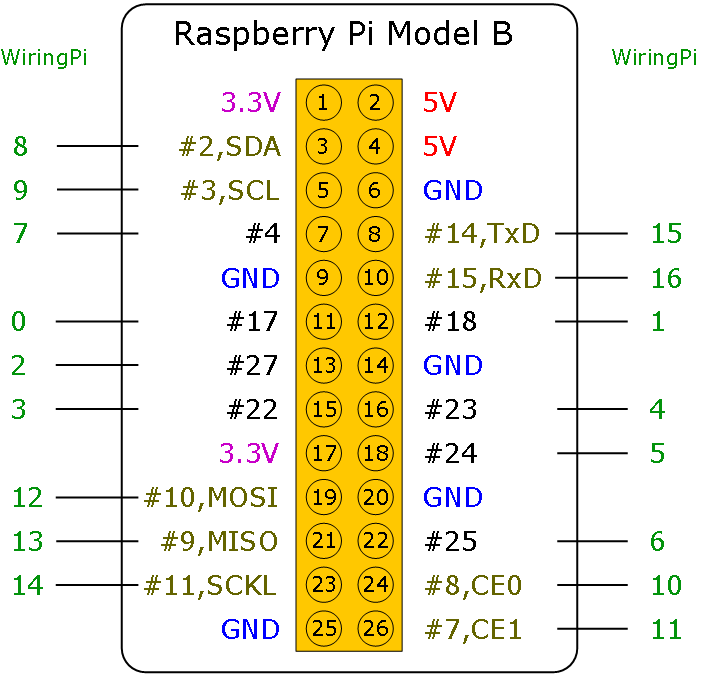
\includegraphics[width=175px]{./images/raspberry/pinmapb.png}
    \label{fig:pin_b}
  }
  \hfill
  \subbottom[Model B+]
  {
    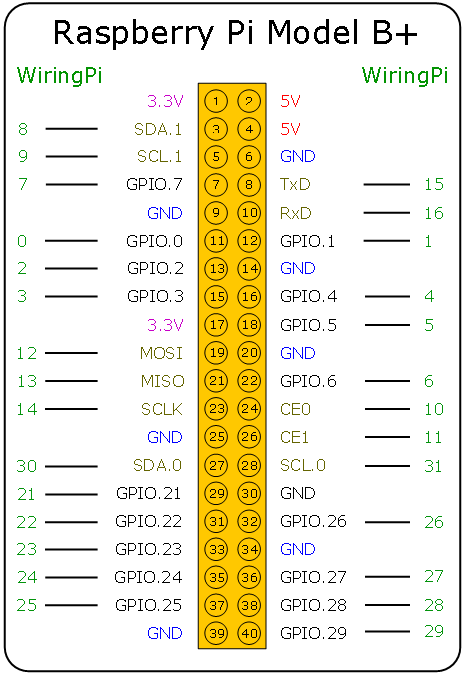
\includegraphics[width=116px]{./images/raspberry/pinmapbp.png}
    \label{fig:pin_bp}
  }
  \caption{Raspberry Pi Pin Map}
  \label{fig:rpi_pin_map}
\end{figure}

\chapter{Application}
본 Chapter에서는 RPi에 연결 가능한 Device 및 Sensor를 이용한 테스트 설명한다. 테스트는 Model B+에서
진행되었으며 Rasbian 과 wiringPi가 기본적으로 설치되어 있어야한다.
\section{Pi Camera}
Raspberry Pi에서 제공하고 있는 카메라는 2종류가 있다. 하나는 일반적으로 사용하는 카메라로 기판 색이 
초록색으로 되어 있으며 가시광선 영역의 파장을 받는다. 다른 하나는 NoIR(No Infrared) 카메라로 기판색이 
검은색이며 가시광선을 포함하여 적외선 영역의 파장까지 인식한다. 즉, NoIR 카메라의 경우 적외선 LED와 
함께 사용하면 어두운 장소에서도 촬영이 가능하다. 반면 낮에는 실제 색감 및 밝기가 일반 카메라와 다르게 
보이는 단점이 있다.
\begin{figure}[h]
  \centering
  \subbottom[Normal Camera] 
  {
    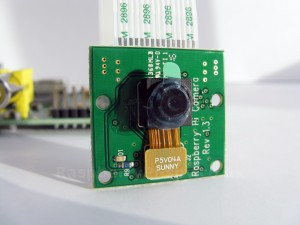
\includegraphics[width=0.47\textwidth]{./images/raspberry/camera.jpg}
    \label{fig:nor_cam}
  }
  \hfill
  \subbottom[NoIR Camera]
  {
    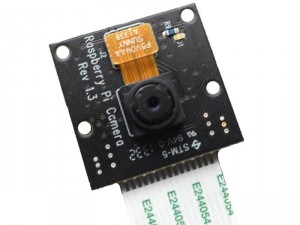
\includegraphics[width=0.47 \textwidth]{./images/raspberry/noircamera.jpg}
    \label{fig:noir_cam}
  }
  \caption{Raspberry Pi Camera Module}
  \label{fig:rpi_cam}
\end{figure}

\subsection{Installation}
RPi 카메라 모듈은 Figure \ref{fig:ist_cam}과 같이 Camera 전용 Port를 사용하며 RPi Configuration
을 통해 Port를 활성화 시켜 준다.
\begin{figure}[h]
\centering
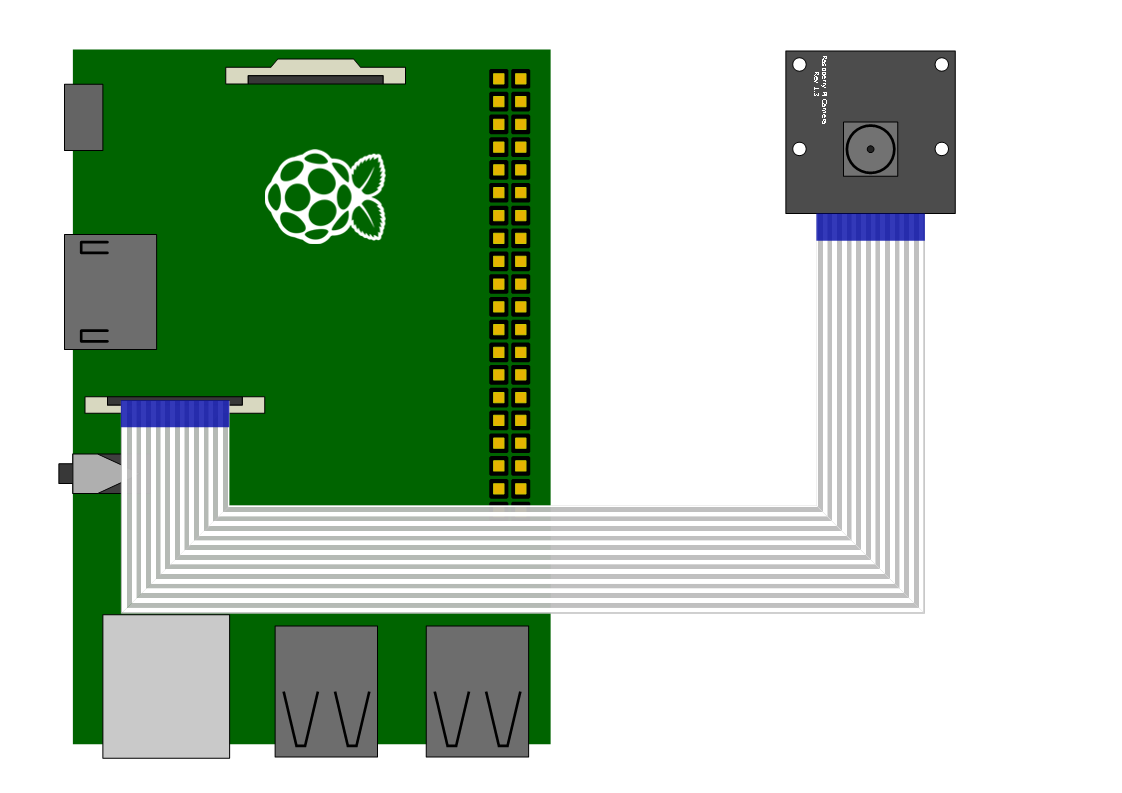
\includegraphics[width=1\textwidth]{./images/raspberry/pi_camera_setting.png}
\caption{Camera Installation}
\label{fig:ist_cam}
\end{figure}
\begin{lstlisting}[style=termstyle]
pi@raspberry# sudo raspi-config
\end{lstlisting}
\begin{figure}
\centering
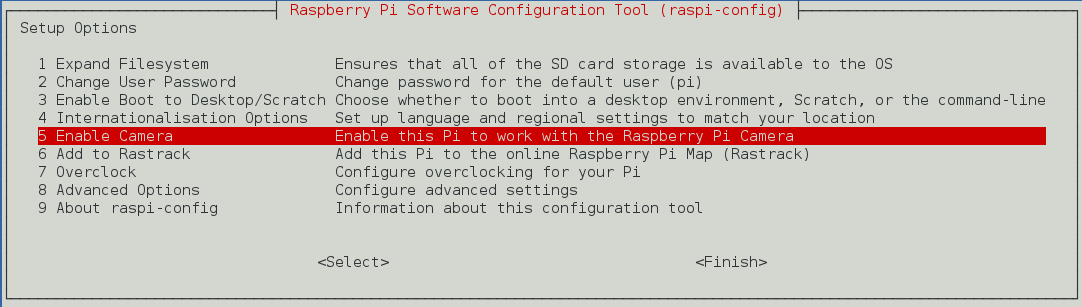
\includegraphics[width=1\textwidth]{./images/raspberry/enable_camera.png}
\caption{Camera Installation}
\label{fig:en_cam}
\end{figure}
\begin{figure}[!htb]
\centering
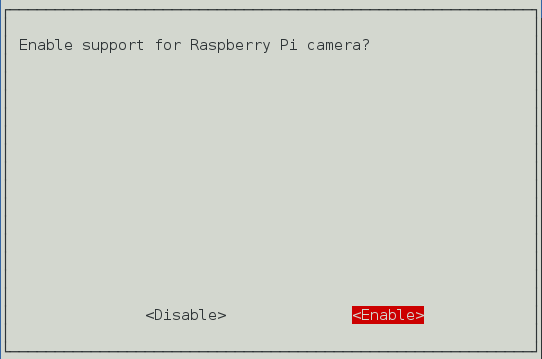
\includegraphics[width=1\textwidth]{./images/raspberry/enable_camera_sel.png}
\caption{Camera Installation}
\label{fig:sel_en_cam}
\end{figure}
설정을 마쳤으면 재부팅 한다.
\begin{lstlisting}[style=termstyle]
pi@raspberry# sudo reboot
\end{lstlisting}
\subsection{Test}
기본적인 카메라 작동은 Shell Command를 사용하며, 보다 다양한 기능의 작동은 Raspberry Pi홈페이지
\cite{PICAM}를 참고하기 바란다.
사진 캡쳐는 raspitill을 사용한다.
\begin{lstlisting}[style=termstyle]
pi@raspberry# raspistill -o cam.jpg
\end{lstlisting}
상하 좌우 반전을 하고 싶으면 vf, hf 옵션을 설정한다.
\begin{lstlisting}[style=termstyle]
pi@raspberry# raspivid -vf -hf -o cam2.jpg
\end{lstlisting}
동영상 촬영은 raspivid를 사용한다.
\begin{lstlisting}[style=termstyle]
pi@raspberry# raspivid -o vid.h264
\end{lstlisting}
t옵션을 사용하면 시간 설정이 가능하다.(기본은 5초) 다음은 10초동안 촬영한다.
\begin{lstlisting}[style=termstyle]
pi@raspberry# sudo raspi-config
\end{lstlisting}
카메라가 작동할 때 LED가 켜지지 않게 하려면 /boot/config.txt 파일에 disable\_camera\_led=1을 
추가한 후 재부팅 한다.
\begin{lstlisting}[style=termstyle]
...
...
...

# NOOBS Auto-generated Settings:
hdmi_force_hotplug=1
config_hdmi_boost=4
overscan_left=24
overscan_right=24
overscan_top=16
overscan_bottom=16
disable_overscan=0
start_x=1
gpu_mem=128
disable_camera_led=1
\end{lstlisting}
\subsection{Web Streaming}
mjpg streamer Library를 이용하면 Web Streaming을 통해 영상을 볼 수 있다. Library를 설치하기 앞서
Web Streaming에 필요한 파일을 설치한다.
\begin{lstlisting}[style=termstyle]
pi@raspberry# sudo apt-get install git cmake libjpeg8-dev imagemagick -y
\end{lstlisting}
파일 설치가 완료되면 videodev.h 헤더파일을 videodev2.h파일로 링크한다.
\begin{lstlisting}[style=termstyle]
pi@raspberry# sudo ln -s /usr/include/linux/videodev2.h /usr/include/linux/videodev.h
\end{lstlisting}
기본 준비가 끝났으면 git에서 mjpg streamer를 복사한다.
\begin{lstlisting}[style=termstyle]
pi@raspberry# git clone https://github.com/jacksonliam/mjpg-streamer
\end{lstlisting}
mjpg-streamer/mjpg-streamer-experimental 폴더로 이동한 후 make를 실행한다.
\begin{lstlisting}[style=termstyle]
pi@raspberrypi# cd mjpg-streamer/mjpg-streamer-experimental
pi@raspberrypi:/mjpg-streamer/mjpg-streamer-experimental# make
\end{lstlisting}
make가 완료되면 다음과 같은 실행 스크립트를 만든다.
\begin{lstlisting}[style=termstyle]
export STREAMER_PATH=$HOME/mjpg-streamer/mjpg-streamer-experimental
export LD_LIBRARY_PATH=$STREAMER_PATH
$STREAMER_PATH/mjpg_streamer -i "input_raspicam.so -x 640 -y 480 -fps 30" -o "output_http.so -w $STREAMER_PATH/www"
\end{lstlisting}
마지막으로 스크립트를 실행 한다.
\begin{lstlisting}[style=termstyle]
pi@raspberrypi# sh mjpg.sh
MJPG Streamer Version: svn rev:
 DBG(/home/pi/mjpg-streamer/mjpg-streamer-experimental/plugins/input_raspicam/input_raspicam.c, input_init(), 118): argv[0]=raspicam 
input plugin
 DBG(/home/pi/mjpg-streamer/mjpg-streamer-experimental/plugins/input_raspicam/input_raspicam.c, input_init(), 118): argv[1]=-x
 DBG(/home/pi/mjpg-streamer/mjpg-streamer-experimental/plugins/input_raspicam/input_raspicam.c, input_init(), 118): argv[2]=640
 DBG(/home/pi/mjpg-streamer/mjpg-streamer-experimental/plugins/input_raspicam/input_raspicam.c, input_init(), 118): argv[3]=-y
 DBG(/home/pi/mjpg-streamer/mjpg-streamer-experimental/plugins/input_raspicam/input_raspicam.c, input_init(), 118): argv[4]=480
 DBG(/home/pi/mjpg-streamer/mjpg-streamer-experimental/plugins/input_raspicam/input_raspicam.c, input_init(), 118): argv[5]=-fps
 DBG(/home/pi/mjpg-streamer/mjpg-streamer-experimental/plugins/input_raspicam/input_raspicam.c, input_init(), 118): argv[6]=30
 DBG(/home/pi/mjpg-streamer/mjpg-streamer-experimental/plugins/input_raspicam/input_raspicam.c, input_init(), 175): case 2,3
 DBG(/home/pi/mjpg-streamer/mjpg-streamer-experimental/plugins/input_raspicam/input_raspicam.c, input_init(), 181): case 4,5
 DBG(/home/pi/mjpg-streamer/mjpg-streamer-experimental/plugins/input_raspicam/input_raspicam.c, input_init(), 187): case 6, 7
 i: fps.............: 30
 i: resolution........: 640 x 480
 i: camera parameters..............:

Sharpness 0, Contrast 0, Brightness 50
Saturation 0, ISO 400, Video Stabilisation No, Exposure compensation 0
Exposure Mode 'auto', AWB Mode 'auto', Image Effect 'none'
Metering Mode 'average', Colour Effect Enabled No with U = 128, V = 128
Rotation 0, hflip No, vflip No
 o: www-folder-path...: /home/pi/mjpg-streamer/mjpg-streamer-experimental/www/
 o: HTTP TCP port.....: 8080
 o: username:password.: disabled
 o: commands..........: enabled
 i: Starting Camera
 DBG(/home/pi/mjpg-streamer/mjpg-streamer-experimental/plugins/input_raspicam/input_raspicam.c, worker_thread(), 553): Host init, starting mmal 
stuff
 DBG(/home/pi/mjpg-streamer/mjpg-streamer-experimental/plugins/input_raspicam/input_raspicam.c, worker_thread(), 681): Camera enabled, creating 
encoder
Encoder Buffer Size 81920
 DBG(/home/pi/mjpg-streamer/mjpg-streamer-experimental/plugins/input_raspicam/input_raspicam.c, worker_thread(), 764): Encoder enabled, creating 
pool and connecting ports
 DBG(/home/pi/mjpg-streamer/mjpg-streamer-experimental/plugins/input_raspicam/input_raspicam.c, worker_thread(), 880): Starting video o
\end{lstlisting}
스크립트가 실행되면 다음 주소를 통해 영상을 확인할 수 있다.\\
\\
http://[IP Address]:8080 \\
\\
\begin{figure}[h]
\centering
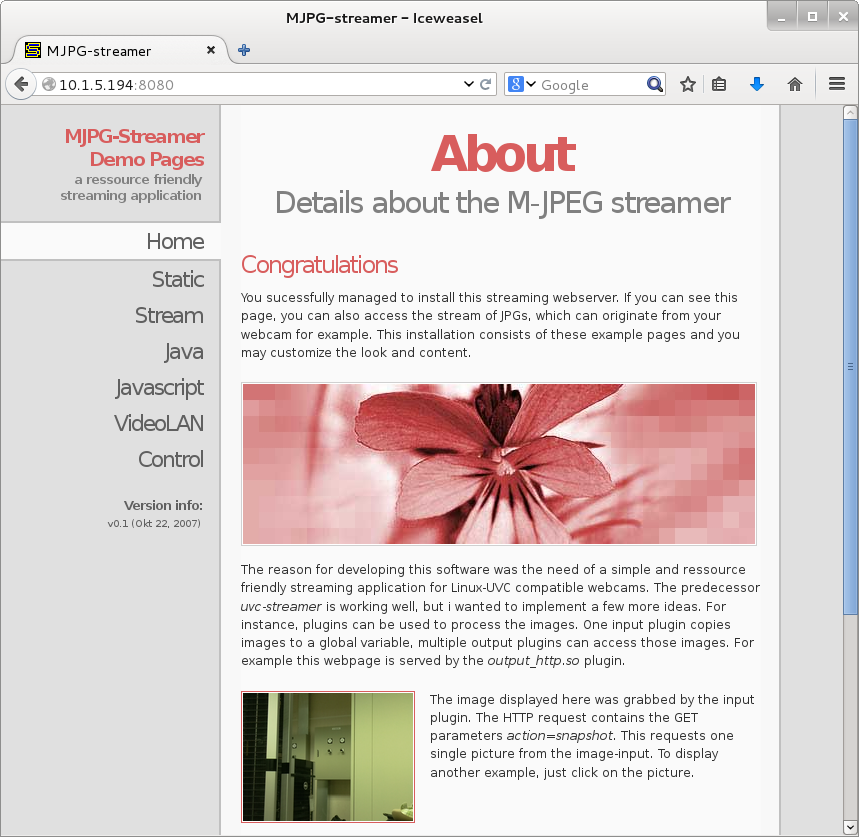
\includegraphics[width=1\textwidth]{./images/raspberry/web_streaming.png}
\caption{Camera Installation}
\label{fig:web_stream_cam}
\end{figure}

wget명령어를 사용하면 Web Streaming으로 부터 이미지를 저장할 수 있다.
\begin{lstlisting}[style=termstyle]
scwook@scwook# wget http://10.1.5.194:8080/?action=snapshot -O image.jpg
\end{lstlisting}
Script를 만들면 주기적으로 이미지를 저장할 수 있다. 다음은 2초 간격으로 이미지를 저장하는 script이다.
\begin{lstlisting}[style=termstyle]
while :
do
	DATE=$(date +"%Y-%m-%d_%H%M%S")
	wget -nv http://10.1.5.194:8080/?action=snapshot -O ./camera/$DATE.jpg
	sleep 2
done
\end{lstlisting}
camera 폴더를 만들고 script를 실행한다.
\begin{lstlisting}[style=termstyle]
scwook@scwook# mkdir camera
scwook@scwook# sh capture.sh
\end{lstlisting}
mencoder를 이용하면 앞서 만든 여러장의 이미지를 하나의 Time-Lapse 동영상으로 만들 수 있다.
파일을 만들기 전에 우선 mencoder를 설치한다.
\begin{lstlisting}[style=termstyle]
scwook@scwook# sudo aptitude install mencoder
\end{lstlisting}
동영상으로 만들 이미지 리스트를 stills.txt 파일로 dump 시킨다.
\begin{lstlisting}[style=termstyle]
scwook@scwook# ls *.jpg > stills.txt
\end{lstlisting}
mencoder를 이용하여 이미지들을 동영상으로 변환 한다.
\begin{lstlisting}[style=termstyle]
scwook@scwook# mencoder -nosound -ovc lavc -lavcopts vcodec=mpeg4:aspect=4/3:vbitrate=8000000 -vf scale=640:480 -o timelapse.avi -mf type=jpeg:fps=24 mf://@stills.txt
\end{lstlisting}
\section{GPIO}\label{sec:gpioApp}
\subsection{LED and Button Test}
버튼을 누르면 LED가 켜지는 테스트를 해보자. 그림\ref{fig:gpio_in_out}과 같은 회로를 구성한다.
\begin{figure}[!htb]
\centering
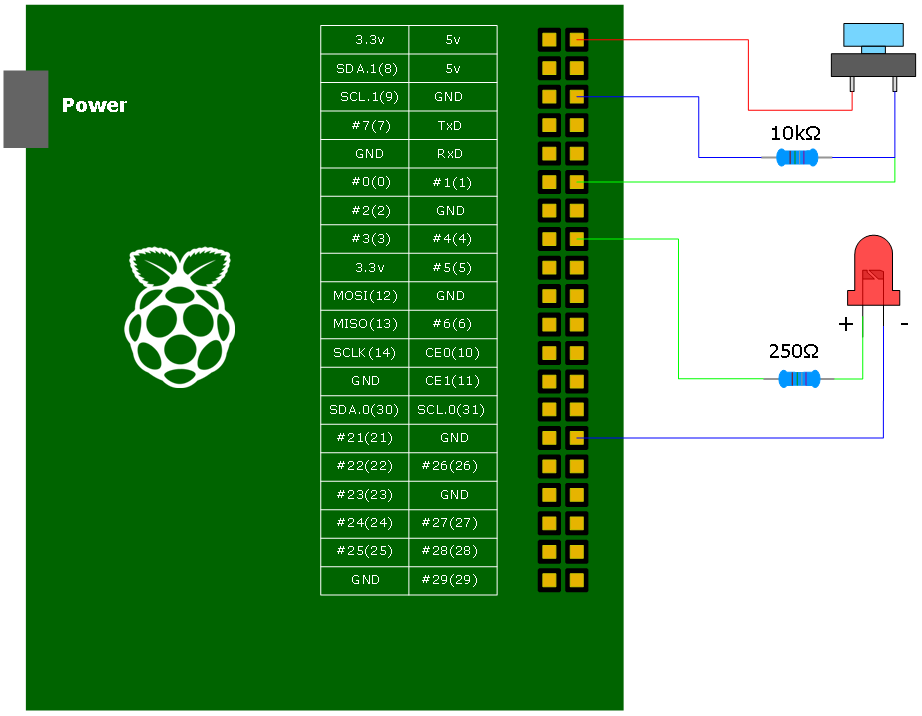
\includegraphics[width=1\textwidth]{./images/raspberry/ledbuttontest.png}
\caption{GPIO In/Out Test}
\label{fig:gpio_in_out}
\end{figure}
소스코드는 다음과 같다.
\begin{lstlisting}[style=termstylenumber, caption={gpio.c}, label={list:gpioTestCode}]
#include <stdio.h>
#include <wiringPi.h>

#define LED 4
#define BUTTON 1

int main(void)
{
  if(wiringPiSetup() == -1)
    return 1;

  pinMode(LED, OUTPUT);
  pinMode(BUTTON, INPUT);

  digitalWrite(LED, 0);
  int input = 0;

  for(;;)
  {
    if(digitalRead(BUTTON))
      digitalWrite(LED, 1);
    else
      digitalWrite(LED, 0); 

    delay(100);
  }

  return 0;
}
\end{lstlisting}
위 코드에서 pinMode함수를 통해 LED는 4번 Output, Button은 1번 Input으로 설정했음을 알 수 있다. 따라서
Button을 누르면 1번 Pin이 High 상태가 되고 이 값은 digitalRead함수를 통해 읽어진다. 반대로 digitalWrite
함수는 설정된 Pin 상태를 1(High) 또는 0(Low)상태로 설정할 수 있다. 위 코드에서는 Button의 상태에 따라
LED가 ON/OFF됨을 알 수 있다.\\

코드를 실행하기 위해 wiringPi Library를 추가한 후 컴파일 한다. 최종적으로 프로그램을 실행한 상태에서
Button을 눌렀을 때 LED에 불이 들어오는지 확인한다.
\begin{lstlisting}[style=termstyle]
pi@raspberrypi# gcc -o buttonTest buttonTest.c -lwiringPi
pi@raspberrypi# sudo ./buttonTest
\end{lstlisting}
\subsection{PIR Motion Sensor}
PIR Motion 센서는 적외선을 이용하여 움직임을 감지하는 센서로 센서의 Detection Area에 움직임이 감지될
경우 3V의 출력을 내보낸다. 따라서 출력신호를 GPIO에 연결하여 센서의 상태를 읽을 수 있다. 센서에 대한 
기본 사양은 다음과 같다.
\begin{itemize}
\item Input Voltage: 3.3 ~ 5V, 6V Maximum
\item Working Current: 15uA
\item Working Temperature: -20 ~ 85 ℃
\item Output Voltage: High 3V, low 0V
\item Output Delay Time(High Level): About 2.3 to 3 Seconds
\item Detection angle: 100 °
\item Detection distance: 7 meters
\item Output Indicator LED(When output HIGH, it will be ON)
\item Pin limit current: 100mA
\end{itemize}

테스트를 위해 그림\ref{fig:pir_test}과 같은 회로를 구성한다.
\begin{figure}[!htb]
\centering
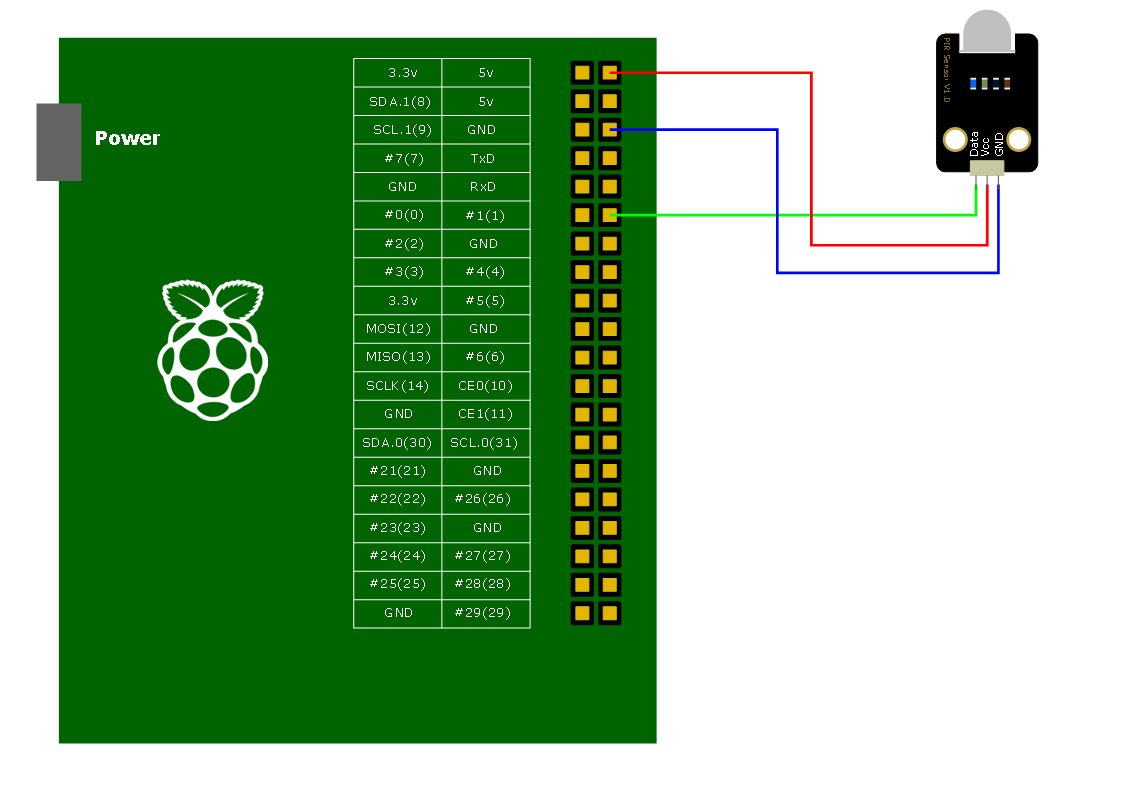
\includegraphics[width=1\textwidth]{./images/raspberry/pir_test.png}
\caption{PIR Motion Sensor Test}
\label{fig:pir_test}
\end{figure}
소스코드는 다음과 같다.
\begin{lstlisting}[style=termstylenumber, caption={pri.c}, label={list:priTestCode}]
#include <stdio.h>
#include <wiringPi.h>

#define PIR 1

int main(void)
{
  if(wiringPiSetup() == -1)
    return 1;

  pinMode(PIR, INPUT);

  int input = 0;

  for(;;)
  {
    if(digitalRead(PIR))
      printf("Motion Detected!\n");

    delay(100);
  }

  return 0;
}
\end{lstlisting}
PIR Motion Sensor는 3V의 출력 신호가 나온다. 따라서 pinMode를 Input으로 설정하였으며 digitalRead 함수를
통해 값을 Monitoring한다. 위 코드에서는 Motion이 감지될 때 "Motion Detected!" 문자가 출력되어 Sensor의
작동을 확인할 수 있다. 
코드를 실행하기 위해 wiringPi Library를 추가한 후 컴파일 한다. 최종적으로 프로그램을 실행한 상태에서
Motion이 감지되는지 확인한다.
\begin{lstlisting}[style=termstyle]
pi@raspberrypi# gcc -o pir pir.c -lwiringPi
pi@raspberrypi# sudo ./pir
\end{lstlisting}
\section{Humidity and Temperature Sensor}
\subsection{DHT11}\label{subsec:dht11App}
DHT11 센서를 이용하여 온도와 습도를 읽어 보자. 그림\ref{fig:dht11_test}와 같은 회로를 구성한다.
\begin{figure}[!htb]
\centering
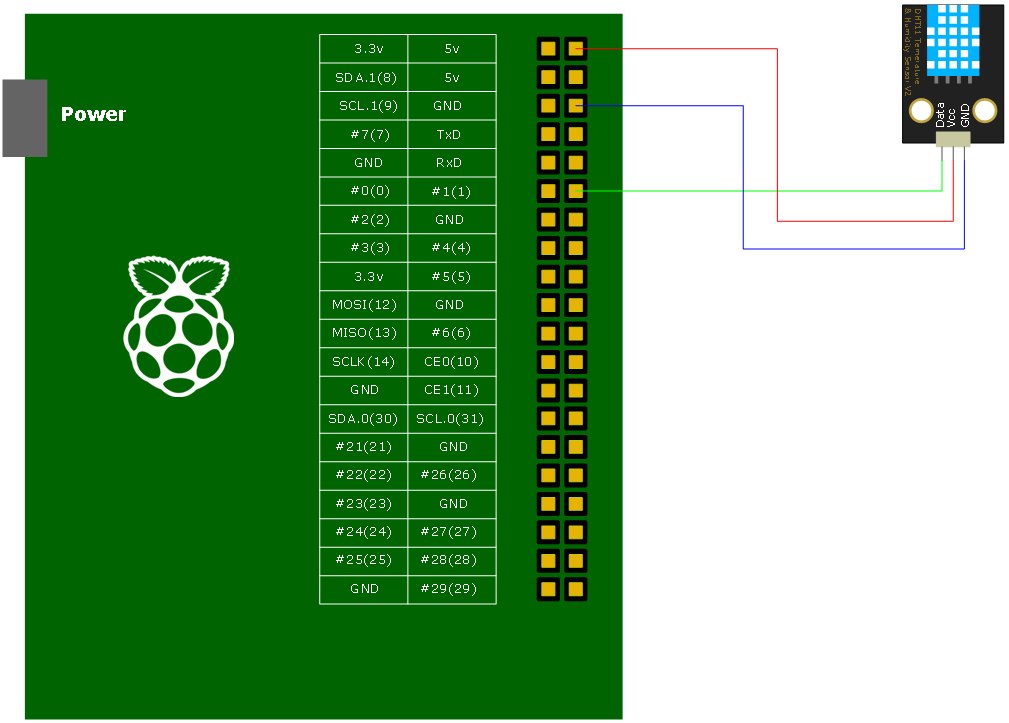
\includegraphics[width=1\textwidth]{./images/raspberry/dht11test.png}
\caption{DHT11 Sensor Test}
\label{fig:dht11_test}
\end{figure}
소스코드는 다음과 같다.
\begin{lstlisting}[style=termstylenumber, caption={dht11.c}, label={list:dhtTestCode}]
#include <wiringPi.h>  
#include <stdio.h>  
#include <stdlib.h>  
#include <stdint.h> 

#define MAX_TIME 85  
#define DHT11PIN 1

int dht11_val[5]={0,0,0,0,0};  

void dht11_read_val()  
{  
uint8_t lststate=HIGH;  
  uint8_t counter=0;  
  uint8_t j=0,i;  

  for(i=0;i<5;i++)  
     dht11_val[i]=0;  

  pinMode(DHT11PIN,OUTPUT);  
  digitalWrite(DHT11PIN,LOW);  

  delay(18);  

  digitalWrite(DHT11PIN,HIGH);  

  delayMicroseconds(40);  

  pinMode(DHT11PIN,INPUT);  
  for(i=0;i<MAX_TIME;i++)  
  {  
    counter=0;  
    while(digitalRead(DHT11PIN)==lststate){  
      counter++;  
      delayMicroseconds(1);  
      if(counter==255)  
	break;  
    }  

    lststate=digitalRead(DHT11PIN);  

    if(counter==255)  
       break;  

    // top 3 transistions are ignored  
    if((i>=4)&&(i%2==0)){  
      dht11_val[j/8]<<=1;  
      if(counter>16)  
	dht11_val[j/8]|=1;  
      j++;  
    }  
  }  

  // verify cheksum and print the verified data  
  if((j>=40)&&(dht11_val[4]==((dht11_val[0]+dht11_val[1]+dht11_val[2]+dht11_val[3])& 0xFF)))  
  {  
    farenheit=dht11_val[2]*9./5.+32;  
    printf("H = %d.%d\nT = %d.%d\n",dht11_val[0],dht11_val[1],dht11_val[2],dht11_val[3]);  
  }  
  else  
    printf("Invalid Data!!\n");  
}  
  
int main(void)  
{  
  if(wiringPiSetup()==-1)  
    exit(1);  
  
  while(1)  
  {  
     dht11_read_val();  
       delay(1000);  
  }  
  
  return 0; 
}
\end{lstlisting}
read_dht11_val함수는 센서로 부터 data를 읽어 온습도값을 출력해주는 함수로 
컴파일 후 실행한다.
\begin{lstlisting}[style=termstyle]
pi@raspberrypi# gcc -o dht11 dht11.c -lwiringPi
pi@raspberrypi# sudo ./dht11
\end{lstlisting}
온습도 값이 출력되면 성공!
\subsection{DS1820}\label{subsec:ds1820App}
DS1820 센서를 이용하여 온도를 읽어 보자.
\begin{figure}[!htb]
\centering
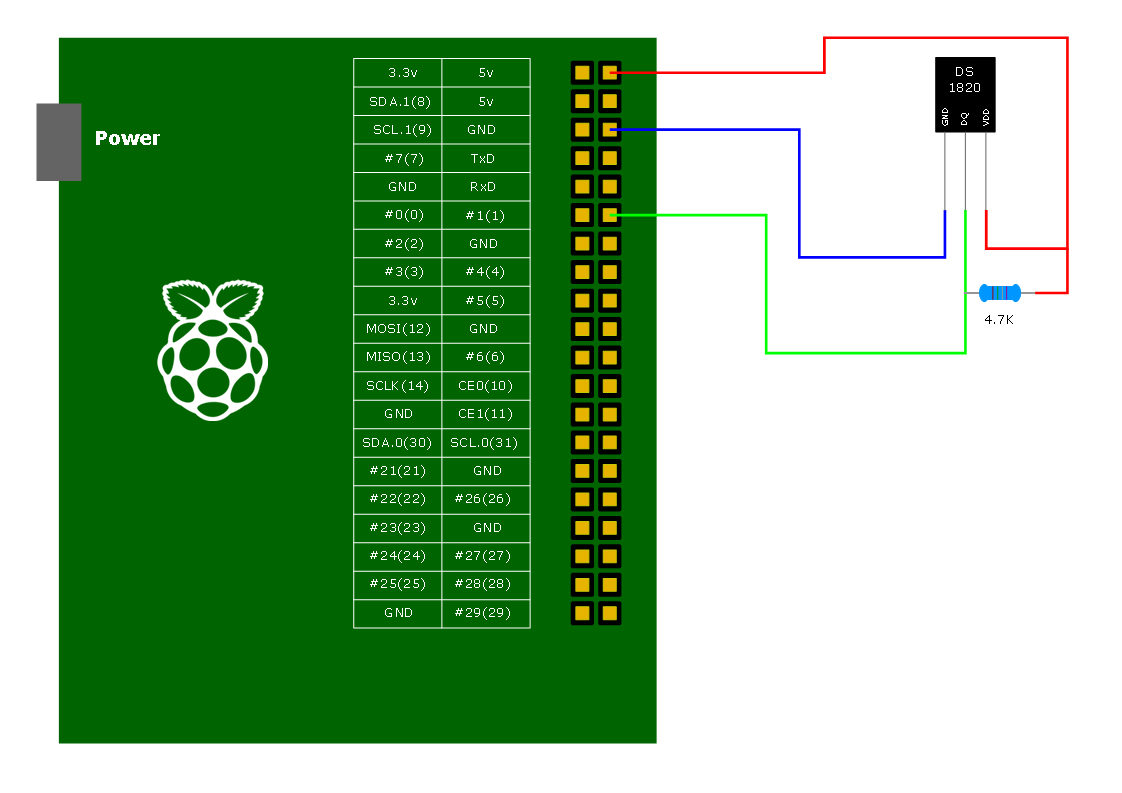
\includegraphics[width=1\textwidth]{./images/raspberry/ds1820_test.png}
\caption{DS1820 Temperature Sensor Test}
\label{fig:ds1820_test}
\end{figure}
소스코드는 다음과 같다.
\begin{lstlisting}[style=termstylenumber, caption={ds1820.c}, label={list:ds1820TestCode}]
#include <stdio.h>
#include <string.h>
#include <stdlib.h>
#include <stdint.h>

#include <wiringPi.h>

#define PIN_NUM 1

float ds1820_read();
int onewire_reset();
void onewire_write(uint8_t data);
void onewire_write_bit(int bit);
uint8_t onewire_read();
int onewire_read_bit();
uint8_t crc_read();
uint8_t crc_cal(uint8_t crc, uint8_t data);

int main()
{
  if(wiringPiSetup() == -1)
    return 1;

  float temp = 0.0f;

  while(1)
  {
    temp = ds1820_read();
    printf("%.1f\n", temp);

   delay(1000);
  }
}
float ds1820_read()
{
  uint8_t busy = 1;

  onewire_reset();
  onewire_write(0xCC);
  onewire_write(0x44);

  delay(750);
  while(busy == 0)
  {
    busy = onewire_read();
    printf("busy: %d\n", busy);
  }

  onewire_reset();
  onewire_write(0xCC);
  onewire_write(0xBE);

  uint8_t lsb, msb, th, tl, reserved1, reserved2, count_remain, count_per_c, crc;
  float real_temp = 0.0f;
  signed char temp_read = 0;

  lsb = onewire_read();
  msb = onewire_read();
  th = onewire_read();
  tl = onewire_read();
  reserved1 = onewire_read();
  reserved2 = onewire_read();
  count_remain = onewire_read();
  count_per_c = onewire_read();
  crc = onewire_read();

  uint8_t data[] = {lsb, msb, th, tl, reserved1, reserved2, count_remain, count_per_c};

  onewire_reset();

  if(crc_read(data) == crc)
  {
    temp_read = (signed char)(lsb>>1);

    if(msb == 255)
      temp_read = temp_read | 0x80;

    real_temp = (float)temp_read + 0.85f - (float)count_remain/(float)count_per_c;
    real_temp = (int)(real_temp * 10) / 10.0f;
  }
  else
    printf("CRC Error  ");

  return real_temp;
}

int onewire_reset()
{
  int result;

  pinMode(PIN_NUM, OUTPUT);

  digitalWrite(PIN_NUM, LOW);
  delayMicroseconds(480);

  pinMode(PIN_NUM, INPUT);
  delayMicroseconds(70);

  result = digitalRead(PIN_NUM);

  delayMicroseconds(410);

  return result;
}

void onewire_write(uint8_t data)
{
  int loop;

  for(loop=0; loop<8; loop++)
  {
    onewire_write_bit(data & 0x01);

    data >>= 1;
  }
}
void onewire_write_bit(int bit)
{
  pinMode(PIN_NUM, OUTPUT);

  if(bit)
  {
    digitalWrite(PIN_NUM, LOW);
    delayMicroseconds(6);
    digitalWrite(PIN_NUM, HIGH);
    delayMicroseconds(64);
  }
  else
  {
    digitalWrite(PIN_NUM, LOW);
    delayMicroseconds(60);
    digitalWrite(PIN_NUM, HIGH);
    delayMicroseconds(10);
  }

}

uint8_t onewire_read()
{
  int loop, result=0;

  for(loop=0; loop<8; loop++)
  {
    result >>= 1;

    if(onewire_read_bit())
      result |= 0x80;
  }

  return result;
}

int onewire_read_bit()
{
  int result;

  pinMode(PIN_NUM, OUTPUT);

  digitalWrite(PIN_NUM, LOW);
  delayMicroseconds(6);

  pinMode(PIN_NUM, INPUT);
  delayMicroseconds(9);

  result = digitalRead(PIN_NUM) & 0x01;
  delayMicroseconds(55);

  return result;
}

uint8_t crc_read(uint8_t *data)
{
 uint8_t i, crc;

 crc = 0x00;

 for(i=0; i<8; i++)
  crc = crc_cal(crc, data[i]);

 return crc;
}

uint8_t crc_cal(uint8_t crc, uint8_t data)
{
  int j;
  for(j=0;j<8;j++) {
      if ((data & 0x01 ) ^ (crc & 0x01)) {
	  // DATA ^ LSB CRC = 1
	  crc = crc>>1;
	  // Set the MSB to 1
	  crc = crc | 0x80;
	  // Check bit 3
	  if (crc & 0x04) {
	      crc = crc & 0xFB; // Bit 3 is set, so clear it
	  } else {
	      crc = crc | 0x04; // Bit 3 is clear, so set it
	  }
	  // Check bit 4
	  if (crc & 0x08) {
	      crc = crc & 0xF7; // Bit 4 is set, so clear it
	  } else {
	      crc = crc | 0x08; // Bit 4 is clear, so set it
	  }
      } else {
	  // DATA ^ LSB CRC = 0
	  crc = crc>>1;
	  // clear MSB
	  crc = crc & 0x7F;
	  // No need to check bits, with DATA ^ LSB CRC = 0, they will remain unchanged
      }
      data = data>>1;
  }

  return crc;
}
\end{lstlisting}
ds1820_read함수는 bit data를 읽어 온도값을 return하는 함수로 크게 다음 4개의 함수를 호출한다.
onewire_reset함수는 command전송하기 위한 초기화 과정을 수행한다. 초기화가 완료되면 
\begin{lstlisting}[style=termstyle]
pi@raspberrypi# gcc -o ds1820 ds1820.c -lwiringPi
pi@raspberrypi# sudo ./ds1820
\end{lstlisting}
온도 값이 출력되면 성공
\section{Dust Sensor}
\subsection{PM1001}\label{subsec:pm1001Test}
PM1001의 경우 UART 통신을 통해 데이터를 전송하므로 Raspberry Pi의 UART 포트와 연결이 가능하다.
센서에 연결하기 전에 \ref{subsec:uartConfig}를 참고하여 UART Consol 설정을 해제한다.
테스트 회로는 그림\ref{fig:pm1001_test}와 같다.
\begin{figure}[!htb]
\centering
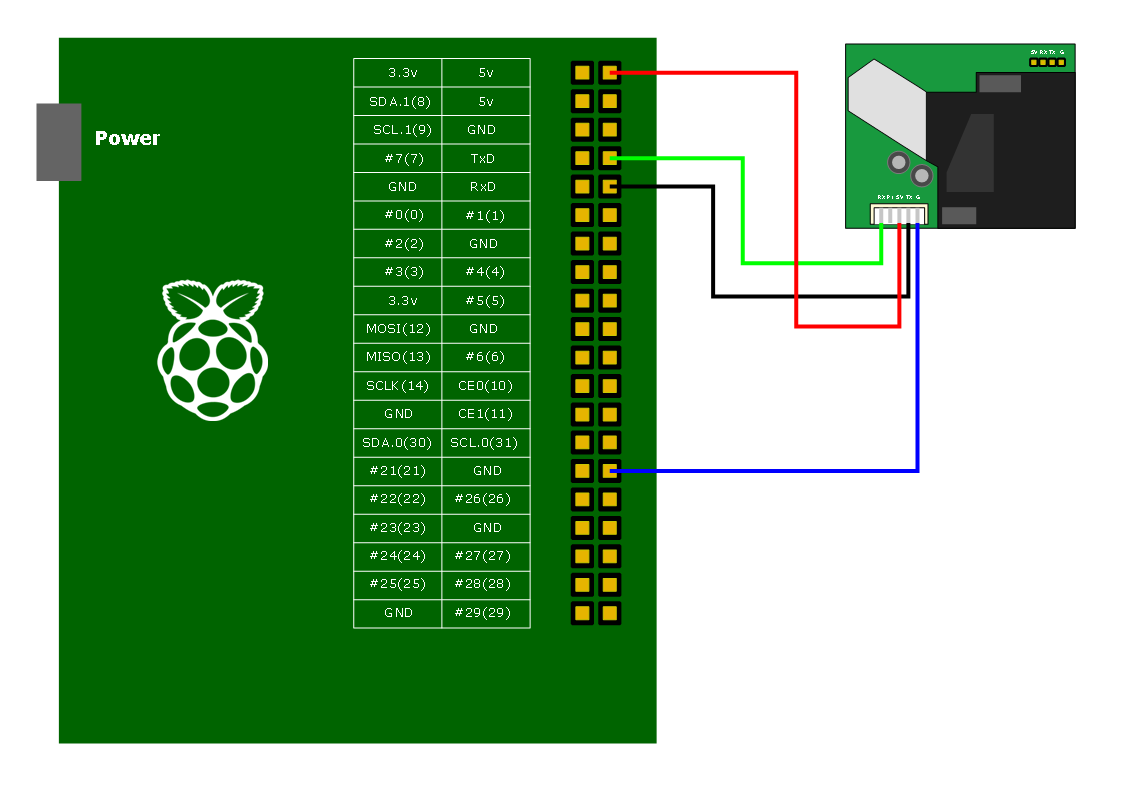
\includegraphics[width=1\textwidth]{./images/epics/PM1001Test.png}
\caption{PM1001 Dust Sensor}
\label{fig:pm1001_test}
\end{figure}
메뉴얼에 따르면 PM1001의 통신 명령어는 다음과 같다.\\
\\
        SEND: [IP] [LB] [CMD] [DF] [CS]\\
\\
        RESPONSE: [ACK] [LB] [CMD] [DF] [CS]\\
\\
여기서 각 명령에 대한 의미는 다음과 같다.\newline
[IP]: address(fixed as 0x11)\newline
[LB]: byte length followed does not include CS\newline
[CMD]: command\newline
[DF]: parameter items with command, optional\newline
[CS]: CS = -(IP + LB + CMD + DF)\newline
[ACK] 0x16 right command\newline
\newline
예를 들어 PM1001로 부터 먼지 값을 읽는 명령어는 다음과 같다.\newline\newline
        SEND: 0X11, 0X01, 0X01, 0XED\newline\newline
        RESPONSE: 0x16, 0x0D, 0x01, 4BytePM값, 4BytePM값, 4BytePM값, [CS]\newline\newline
여기서 PM값은 4Byte(DF0, DF1, DF2, DF3)로 구성된 먼지 데이터 값으로 측정 값은 다음과 같다.\newline\newline
        Measured value = DF0 * 256 * 256 * 256 + DF1 * 256 * 256 + DF2 * 256 + DF3\newline

기본 단위는 PCS/L 로 농도(ug/m³)값으로  변환 하고자 할 경우 다음 식을 사용한다.\newline
\newline
        농도(ug/m³) = ((수량PCS/L값) * 3,528) / 100,000\newline

전체 코드는 다음과 같다.
\begin{lstlisting}[style=termstylenumber, caption={pm1001.c}, label={list:pm1001TestCode}]
#include <stdio.h>
#include <wiringPi.h>
#include <wiringSerial.h>

int main(void)
{
  int fd;

  if((fd = serialOpen("/dev/ttyAMA0", 9600)) < 0)
  {
    printf("Unable to open serial device\n");
    return 1;
  }

  if(wiringPiSetup() == -1)
  {
    printf("Unable to start wiringPi\n");
    return 1;
  }

  serialFlush(fd);

  unsigned char c;
  int df[4];
  int dust;

  c = 0x11;
  serialPutchar(fd, c);

  c = 0x01;
  serialPutchar(fd, c);
  serialPutchar(fd, c);

  c = 0xED;
  serialPutchar(fd, c);

  printf("%d ", serialGetchar(fd));
  printf("%d ", serialGetchar(fd));
  printf("%d ", serialGetchar(fd));

  int i=0, j;
  for(i; i<3; i++)
  {
    j=0;
    for(j; j<4; j++)
      df[j] = serialGetchar(fd);

    dust = df[0]*256*256*256 + df[1]*256*256 + df[2]*256 + df[3];
    printf("%d ", dust);
  }

  printf("%d\n", serialGetchar(fd));
  printf("%d %d %d %d\n", df[0], df[1], df[2], df[3]);

  serialFlush(fd);
  serialClose(fd);

  return 0;
}
\end{lstlisting}
컴파일 후 실행한다.
\begin{lstlisting}[style=termstyle]
pi@raspberrypi# gcc -o pm1001 pm1001.c -lwiringPi
pi@raspberrypi# sudo ./pm1001
\end{lstlisting}
먼지 값이 출력되면 성공
\section{Motor}
\subsection{L298 Dual H-Brdge}
L298 Dual H-Bridge를 이용하여 2Phase Motor를 작동시켜 보자.
그림\ref{fig:l298_test}와 같은 회로를 구성한다.
\begin{figure}[!htb]
\centering
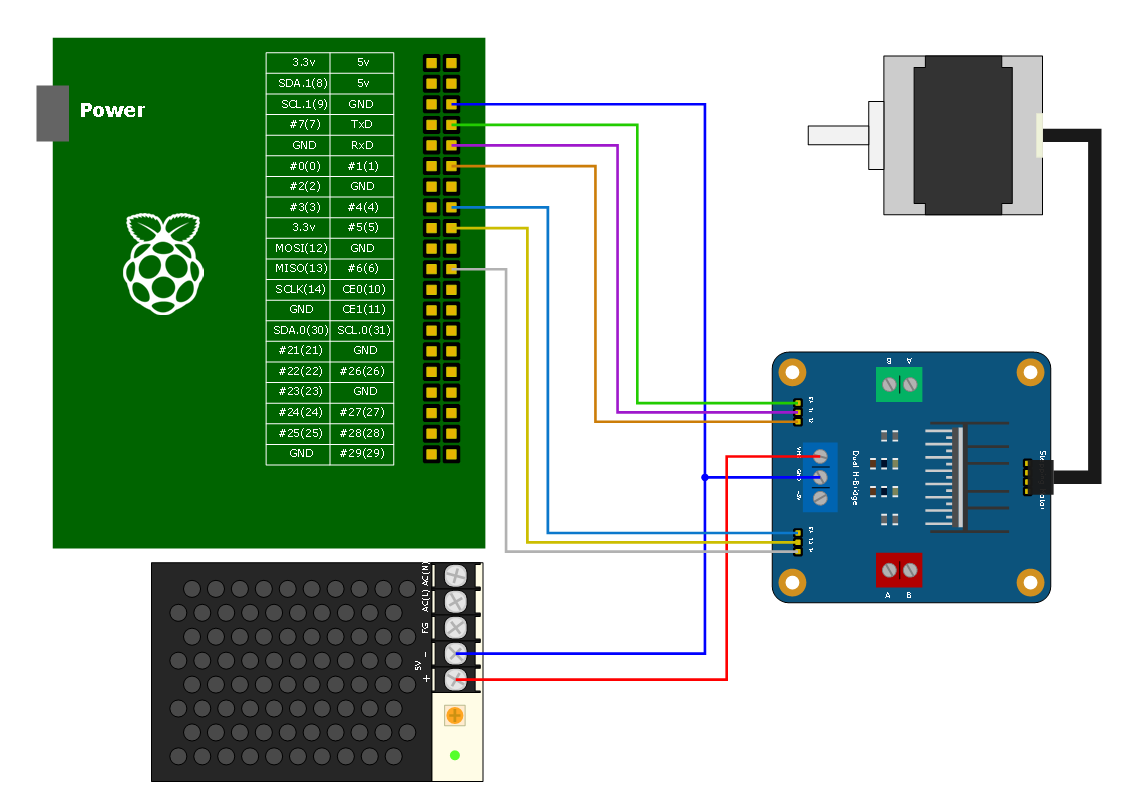
\includegraphics[width=1\textwidth]{./images/raspberry/L298Test.png}
\caption{L298 Dual H-Bridge 2Phase Step Motor}
\label{fig:l298_test}
\end{figure}
소스코드는 다음과 같다.
\begin{lstlisting}[style=termstylenumber, caption={l298.c}, label={list:l298TestCode}]
#include <stdio.h>
#include <wiringPi.h>

#define TRUE 1
#define FALSE 0
#define DELAY 1800

#define EA 15
#define EB 4
#define IN1 16
#define IN2 1
#define IN3 5
#define IN4 6

void setStep(int a, int b, int c, int d)
{
   digitalWrite(IN1, a);
   digitalWrite(IN2, b);
   digitalWrite(IN3, c);
   digitalWrite(IN4, d);
}

int main(void)
{
  if(wiringPiSetup() == -1)
  {
    printf("Init Error\n");
    return 1;
  }

  pinMode(EA, OUTPUT);
  pinMode(IN1, OUTPUT);
  pinMode(IN2, OUTPUT);
  pinMode(EB, OUTPUT);
  pinMode(IN3, OUTPUT);
  pinMode(IN4, OUTPUT);

  digitalWrite(EA, TRUE);
  digitalWrite(EB, TRUE);

  int i;
  int loop;

  for(;;)
  {
    for(i=0; i<500; i++)
    {
      setStep(1,0,1,0);
      delayMicroseconds(DELAY);
      setStep(0,1,1,0);
      delayMicroseconds(DELAY);
      setStep(0,1,0,1);
      delayMicroseconds(DELAY);
      setStep(1,0,0,1);
      delayMicroseconds(DELAY);
    }

    delay(1000);

    for(i=0; i<500; i++)
    {
      setStep(1,0,0,1);
      delayMicroseconds(DELAY);
      setStep(0,1,0,1);
      delayMicroseconds(DELAY);
      setStep(0,1,1,0);
      delayMicroseconds(DELAY);
      setStep(1,0,1,0);
      delayMicroseconds(DELAY);
    }

    delay(1000);

  }

  digitalWrite(EA, FALSE);
  digitalWrite(EB, FALSE);
\end{lstlisting}
위 코드에서 setStep함수는 IN신호를 만드는 함수로 총 4번의 Step이 1Cycle이 된다. 
1Step당 1.8도씩 회전하며 총 회전수는 반복문을 통해 제어 가능하다. 따라서 모터를 1회전 하고자 하면 
반복 횟수를 50(360 / 1.8 / 4)으로 하면 된다. 모터 속도는 DELAY시간에 따라 바뀌는데 시간이 너무 짧은 경우
회전하지 않는다. 모통 모터마다 최대 응답속도가 있으므로 그에 맞게 조절해야 한다. 테스트한 모터의 경우 
1.8ms(대략 167rpm)보다 짧은 경우 불규칙적인 회전을 보인다. Step신호를 반대로 주면 순서가 반대로 
작용하므로 모터 방향이 바뀐다. 모터의 방향은 Step순서를 반대로 하면 된다.
\subsection{MD5-DH14}
MD-DH14 Motor Driver를 이용하여 5Phase Pentagon방식의 Step Motor를 작동시켜 보자.
그림\ref{fig:5phase_test}과 같이 회로를 구성한다.
\begin{figure}[!htb]
\centering
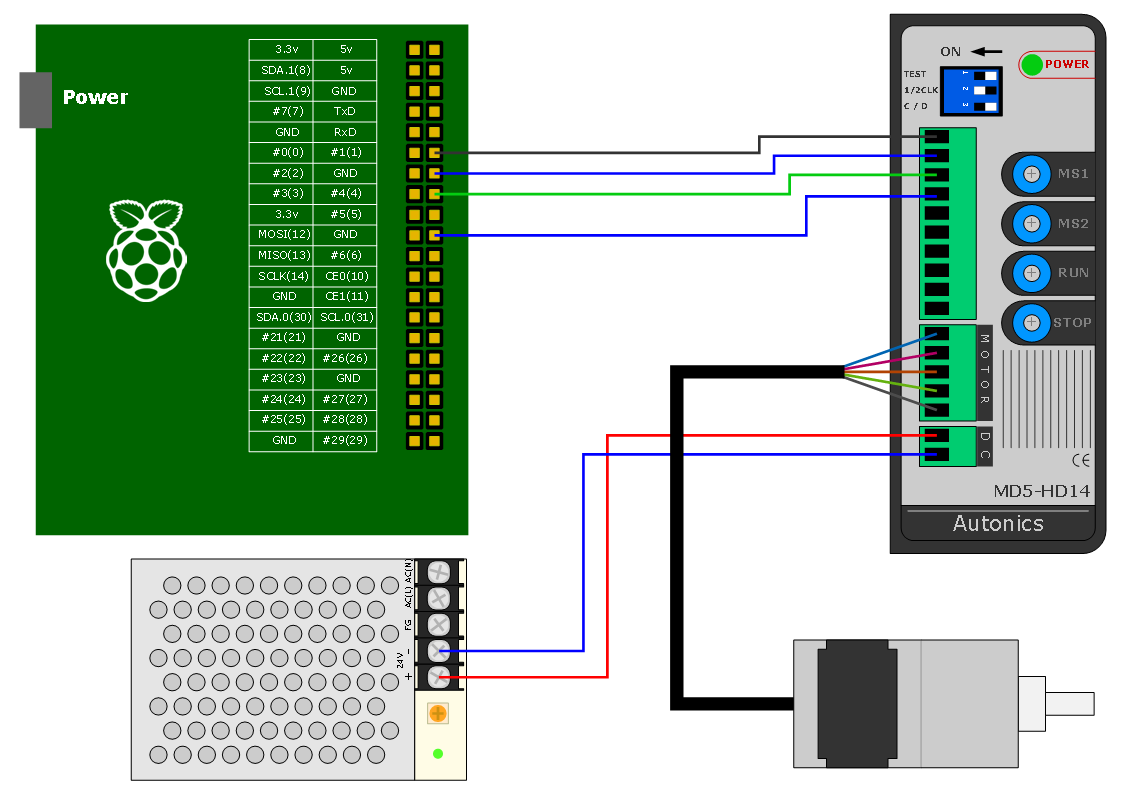
\includegraphics[width=1\textwidth]{./images/raspberry/md5dh14Test.png}
\caption{5Phase Motor Test}
\label{fig:5phase_test}
\end{figure}
소스코드는 다음과 같다.
\begin{lstlisting}[style=termstylenumber, caption={md5dh14.c}, label={list:md5dh14TestCode}]
#include <stdio.h>
#include <wiringPi.h>

#define PULSE 5000

int main(void)
{
  if(wiringPiSetup() == -1)
  {
    printf("Init Error\n");
    return 1;
  }

  pinMode(1, OUTPUT);
  pinMode(4, OUTPUT);

  int pulse;
  for(;;)
  {
    digitalWrite(4, 0);
    for(pulse=0; pulse<PULSE; pulse++)
    {
      digitalWrite(1, 1);
      delayMicroseconds(500);
      digitalWrite(1, 0);
      delayMicroseconds(500);
    }

    digitalWrite(4, 1);
    for(pulse=0; pulse<PULSE; pulse++)
    {
      digitalWrite(1, 1);
      delayMicroseconds(500);
      digitalWrite(1, 0);
      delayMicroseconds(500);
    }
  }
}

\end{lstlisting}
\chapter{EPICS Integration}
여기서는 앞서 테스트한 Sensor 및 Device를 EPICS에 Integration하고 Channel Access를 통해 값을 Monitoring
또는 Control하는 방법에 대하여 기술하였다. 본 Chapter에서 사용된 EPICS는 3.14.12.4 버전이며 전체적으로
다음과 같은 구조를 바탕으로 하고 있다.

\section{Installation}
위 구조에 맞게 EPICS를 설치하기 위해 git으로 부터 script파일을 받는다.
\begin{lstlisting}[style=termstyle]
pi@raspberrypi# git clone https://github.com/jeonghanlee/scripts_for_epics
\end{lstlisting}
\section{Library}
\subsection{synApps}

\section{GPIO}
section\ref{sec:gpioApp}에서 진행하였던 GPIO 테스트를 EPICS로 Integration 하여 테스트해 본다. 최종 목표는
그림\ref{fig:gpio_in_out}과 같이 회로를 구성하고 다음 epics db를 통해 GPIO를 제어하는 것이다.
\begin{lstlisting}[style=termstyle]
record(bi, "inp1")
{
  field(DTYP, "GPIO")
  field(SCAN, "1 second")
  field(INP, "@1")
}

record(bo, "out4")
{
  field(DTYP, "GPIO")
  field(OUT, "@4")
}
\end{lstlisting}
코드 작성에 앞서 테스트 할 기본 폴더 및 EPICS Application 구조를 생성한다.
\begin{lstlisting}[style=termstyle]
pi@ctrlpi3 cd ../epics/R3.14.12.4/siteApps
pi@ctrlpi3 ~/epics/R3.14.12.4/siteApps# mkdir gpio
pi@ctrlpi3 ~/epics/R3.14.12.4/siteApps# cd gpio
pi@ctrlpi3 ~/epics/R3.14.12.4/siteApps/gpio# makeBaseApp.pl -t ioc gpio
pi@ctrlpi3 ~/epics/R3.14.12.4/siteApps/gpio# makeBaseApp.pl -i -t ioc gpio

Using target architecture linux-arm (only one available)
The following applications are available:
    gpio
What application should the IOC(s) boot?
The default uses the IOC's name, even if not listed above.
Application name? gpio
pi@ctrlpi3 ~/epics/R3.14.12.4/siteApps/gpio# ls
conigure  gpioApp  iocBoot Makefile
\end{lstlisting}
gpioApp/src 폴더로 이동한 후 devGPIO.c 파일을 만들어 다음과 같이 코드를 작성한다.
\begin{lstlisting}[style=termstylenumber, caption={devGPIO.c}, label={list:gpioDevCode}]
#include <stdio.h>
#include <string.h>
#include <stdlib.h>

#include <epicsExport.h>
#include <devSup.h>
#include <boRecord.h>
#include <biRecord.h>

#include <wiringPi.h>

static long bo_init_record(boRecord *pbo);
static long bi_init_record(biRecord *pbi);

static long write_bo(boRecord *pbo);
static long read_bi(biRecord *pbi);

struct Pin_Info
{
  int pin_num;
};

static long bo_init_record(boRecord *pbo)
{
  struct Pin_Info *pin_info = malloc(sizeof(struct Pin_Info));

  if(wiringPiSetup() == -1)
    return 1;

  int pin_num = 0;
  pin_num = atoi(pbo->out.value.instio.string);

  pinMode(pin_num, OUTPUT);

  pin_info->pin_num = pin_num;

  pbo->dpvt = pin_info;

  return 0;
}

static long bi_init_record(biRecord *pbi)
{
  struct Pin_Info *pin_info = malloc(sizeof(struct Pin_Info));

  if(wiringPiSetup() == -1)
    return 1;

  int pin_num = 0;
  pin_num = atoi(pbi->inp.value.instio.string);

  pinMode(pin_num, INPUT);

  pin_info->pin_num = pin_num;

  pbi->dpvt = pin_info;

  return 0;
}


static long write_bo(boRecord *pbo)
{
  struct Pin_Info *pin_info = pbo->dpvt;

  int pin = pin_info->pin_num;
  int val = pbo->rval;

  digitalWrite(pin, val);

  return 0;
}

static long read_bi(biRecord *pbi)
{
  struct Pin_Info *pin_info = pbi->dpvt;

  int pin = pin_info->pin_num;
  int val = digitalRead(pin);

  pbi->rval = val;

  return 0;
}

struct
{
  long num;
  DEVSUPFUN     report;
  DEVSUPFUN     init;
  DEVSUPFUN     init_record;
  DEVSUPFUN     get_ioint_info;
  DEVSUPFUN     write_bo;
  DEVSUPFUN     special_linconv;
} devBoGpioAsync = {
  6,
  NULL,
  NULL,
  bo_init_record,
  NULL,
  write_bo,
  NULL
};

struct
{
  long num;
  DEVSUPFUN     report;
  DEVSUPFUN     init;
  DEVSUPFUN     init_record;
  DEVSUPFUN     get_ioint_info;
  DEVSUPFUN     read_bi;
  DEVSUPFUN     special_linconv;
} devBiGpioAsync = {
  6,
  NULL,
  NULL,
  bi_init_record,
  NULL,
  read_bi,
  NULL
};

epicsExportAddress(dset,devBoGpioAsync);
epicsExportAddress(dset,devBiGpioAsync);
\end{lstlisting}
코드 작성이 완료되면 devGPIO.dbd 파일을 만든다.
\begin{lstlisting}[style=termstyle]
device(bo, INST_IO, devBoGpioAsync, "GPIO")
device(bi, INST_IO, devBiGpioAsync, "GPIO")
\end{lstlisting}
앞서 작성한 코드를 Build하기 위해 Makefile에 다음과 같이 추가한다.
\begin{lstlisting}[style=termstyle]
TOP=../..

include $(TOP)/configure/CONFIG

USR_INCLUDES += -I/home/pi/wiringPi/wiringPi
wiringPi_DIR += /home/pi/wiringPi/wiringPi /home/pi/wiringPi/devLib

#----------------------------------------
#  ADD MACRO DEFINITIONS AFTER THIS LINE
#=============================

#=============================
# Build the IOC application

PROD_IOC = gpio
# gpio.dbd will be created and installed
DBD += gpio.dbd

# gpio.dbd will be made up from these files:
gpio_DBD += base.dbd

# Include dbd files from all support applications:
#gpio_DBD += xxx.dbd
gpio_DBD += devGPIO.dbd

# Add all the support libraries needed by this IOC
#gpio_LIBS += xxx
gpio_LIBS += wiringPi

# gpio_registerRecordDeviceDriver.cpp derives from gpio.dbd
gpio_SRCS += gpio_registerRecordDeviceDriver.cpp
gpio_SRCS += devGPIO.c

# Build the main IOC entry point on workstation OSs.
gpio_SRCS_DEFAULT += gpioMain.cpp
gpio_SRCS_vxWorks += -nil-

# Add support from base/src/vxWorks if needed
#gpio_OBJS_vxWorks += $(EPICS_BASE_BIN)/vxComLibrary

# Finally link to the EPICS Base libraries
gpio_LIBS += $(EPICS_BASE_IOC_LIBS)

#===========================

include $(TOP)/configure/RULES
#----------------------------------------
#  ADD RULES AFTER THIS LINE
\end{lstlisting}
db파일을 만들기 위해 gpioApp/Db 폴더로 이동한 후 다음과 같은 gpio.db 파일을 만든다. 
\begin{lstlisting}[style=termstyle]
record(bi, "inp1")
{
  field(DTYP, "GPIO")
  field(SCAN, "1 second")
  field(INP, "@1")
}

record(bo, "out4")
{
  field(DTYP, "GPIO")
  field(OUT, "@4")
}
\end{lstlisting}
gpio.db에서는 GPIO 1번을 입력으로 4번을 출력으로 설정했음을 알 수있다. 
Makefile에 db파일을 추가해 준다.
\begin{lstlisting}[style=termstyle]
TOP=../..
include $(TOP)/configure/CONFIG
#----------------------------------------
#  ADD MACRO DEFINITIONS AFTER THIS LINE

#----------------------------------------------------
#  Optimization of db files using dbst (DEFAULT: NO)
#DB_OPT = YES

#----------------------------------------------------
# Create and install (or just install) into /db
# databases, templates, substitutions like this
#DB += xxx.db
DB += gpio.db

#----------------------------------------------------
# If .db template is not named *.template add
# _template = 

include $(TOP)/configure/RULES
#----------------------------------------
#  ADD RULES AFTER THIS LINE
\end{lstlisting}
마지막으로 앞서 작성한 파일들을 컴파일 하기 위해 gpio폴더로 이동한 후 make를 실행한다.
\begin{lstlisting}[style=termstyle]
pi@ctrlpi3 ~/epics/R3.14.12.4/siteApps/gpio# make
\end{lstlisting}
make가 완료되면 bin/linux-arm 폴더에 gpio 파일과 db 폴더에 gpio.db 파일이 만들어 진다.
이제 ioc를 실행시키기 위해 iocBoot/iocgpio 폴더로 이동 후 st.cmd파일에 gpio.db를 Load하는 코드를 
추가해 준다.
\begin{lstlisting}[style=termstyle]
#!../../bin/linux-arm/gpio

## You may have to change gpio to something else
## everywhere it appears in this file

< envPaths

cd ${TOP}

## Register all support components
dbLoadDatabase "dbd/gpio.dbd"
gpio_registerRecordDeviceDriver pdbbase

## Load record instances
#dbLoadTemplate "db/userHost.substitutions"
#dbLoadRecords "db/dbSubExample.db", "user=piHost"
dbLoadRecords "db/gpio.db"

## Set this to see messages from mySub
#var mySubDebug 1

## Run this to trace the stages of iocInit
#traceIocInit

cd ${TOP}/iocBoot/${IOC}
iocInit

## Start any sequence programs
#seq sncExample, "user=piHost"
\end{lstlisting}
마지막으로 st.cmd파일을 실행파일로 변경한 후 실행시킨다.
\begin{lstlisting}[style=termstyle]
pi@ctrlpi3 ~/epics/R3.14.12.4/siteApps/gpio/iocBoot/iocdht11 $ chmod 755 st.cmd
pi@ctrlpi3 ~/epics/R3.14.12.4/siteApps/gpio/iocBoot/iocdht11 $ sudo ./st.cmd
\end{lstlisting}
output 테스트를 위해 다음과 같이 out4 출력값을 1로 하고 LED에 불이 들어오는지 확인한다.
\begin{lstlisting}[style=termstyle]
epics> dbpf out4 1
\end{lstlisting}
input 테스트는 버튼을 눌렀을 때 inp1 값을 읽어 확인한다.
\begin{lstlisting}[style=termstyle]
epics> dbpr inp1
ASG:                DESC:               DISA: 0             DISP: 0             
DISV: 1             NAME: gpio:inp1     RVAL: 0             SEVR: NO_ALARM      
STAT: NO_ALARM      SVAL: 0             TPRO: 0             VAL: 1
\end{lstlisting}
\section{Dust Sensor}
\subsection{PM1001}
section\ref{subsec:pm1001Test}에서 진행하였던 PM1001 Sensor를 EPICS로 Integration 하여 테스트해 본다.
최종 목표는 그림\ref{fig:pm1001_test}와 같이 회로를 구성하고 다음 epics db를 통해 먼지값을 읽는것이다.
\begin{lstlisting}[style=termstyle]
record(ai,"PI:DUST")
{
  field(DTYP, "stream")
  field(INP, "@sensor.proto get_dust UART")
  field(SCAN, "1 second")
}
\end{lstlisting}
코드 작성에 앞서 기본 폴더 및 EPICS Application 구조를 생성한다.
\begin{lstlisting}[style=termstyle]
pi@raspberrypi ~/epics/R3.14.12.4 $ cd siteApps
pi@raspberrypi ~/epics/R3.14.12.4/siteApps $ mkdir pm1001
pi@raspberrypi ~/epics/R3.14.12.4/siteApps $ cd pm1001
pi@raspberrypi ~/epics/R3.14.12.4/siteApps/pm1001 $ makeBaseApp.pl -t ioc pm1001
pi@raspberrypi ~/epics/R3.14.12.4/siteApps/pm1001 $ makeBaseApp.pl -i -t ioc pm1001
Using target architecture linux-arm (only one available)
The following applications are available:
    pm1001
What application should the IOC(s) boot?
The default uses the IOC's name, even if not listed above.
Application name? pm1001
\end{lstlisting}
pm1001/configure/RELEASE 파일에 asyn과 stream Library위치를 추가해 준다.
\begin{lstlisting}[style=termstyle]
# RELEASE - Location of external support modules
#
# IF YOU MAKE ANY CHANGES to this file you must subsequently
# do a "gnumake rebuild" in this application's top level
# directory.
#
# The build process does not check dependencies against files
# that are outside this application, thus you should do a
# "gnumake rebuild" in the top level directory after EPICS_BASE
# or any other external module pointed to below is rebuilt.
#
# Host- or target-specific settings can be given in files named
#  RELEASE.$(EPICS_HOST_ARCH).Common
#  RELEASE.Common.$(T_A)
#  RELEASE.$(EPICS_HOST_ARCH).$(T_A)
#
# This file should ONLY define paths to other support modules,
# or include statements that pull in similar RELEASE files.
# Build settings that are NOT module paths should appear in a
# CONFIG_SITE file.

TEMPLATE_TOP=$(EPICS_BASE)/templates/makeBaseApp/top

# If using the sequencer, point SNCSEQ at its top directory:
#SNCSEQ=$(EPICS_BASE)/../modules/soft/seq

# EPICS_BASE usually appears last so other apps can override stuff:
EPICS_BASE=/home/pi/epics/R3.14.12.4/base

# Set RULES here if you want to take build rules from somewhere
# other than EPICS_BASE:
#RULES=/path/to/epics/support/module/rules/x-y

ASYN=$(EPICS_PATH)/siteLibs
STREAM=$(EPICS_PATH)/siteLibs
\end{lstlisting}
pm1001App/src 폴더로 이동하면 pm1001Main.cpp와 Makefile이 있다. Makefile에 다음 코드를 추가한다.
\begin{lstlisting}[style=termstyle]
TOP=../..

include $(TOP)/configure/CONFIG
#----------------------------------------
#  ADD MACRO DEFINITIONS AFTER THIS LINE
#=============================

#=============================
# Build the IOC application

PROD_IOC = pm1001
# pm1001.dbd will be created and installed
DBD += pm1001.dbd

# pm1001.dbd will be made up from these files:
pm1001_DBD += base.dbd

# Include dbd files from all support applications:
#pm1001_DBD += xxx.dbd

pm1001_DBD += stream.dbd
pm1001_DBD += drvAsynSerialPort.dbd

# Add all the support libraries needed by this IOC
#pm1001_LIBS += xxx

pm1001_LIBS += stream
pm1001_LIBS += asyn

# pm1001_registerRecordDeviceDriver.cpp derives from pm1001.dbd
pm1001_SRCS += pm1001_registerRecordDeviceDriver.cpp

# Build the main IOC entry point on workstation OSs.
pm1001_SRCS_DEFAULT += pm1001Main.cpp
pm1001_SRCS_vxWorks += -nil-

# Add support from base/src/vxWorks if needed
#pm1001_OBJS_vxWorks += $(EPICS_BASE_BIN)/vxComLibrary

# Finally link to the EPICS Base libraries
pm1001_LIBS += $(EPICS_BASE_IOC_LIBS)

#===========================

include $(TOP)/configure/RULES
#----------------------------------------
#  ADD RULES AFTER THIS LINE
\end{lstlisting}
db파일을 만들기 위해 pm1001App/Db 폴더로 이동한 후 다음과 같은 pm1001.db 파일을 만든다.
\begin{lstlisting}[style=termstyle]
record(ai,"PM1001:DUST")
{
  field(DTYP, "stream")
  field(INP, "@sensor.proto get_dust UART")
  field(SCAN, "1 second")
}
\end{lstlisting}
Makefile에 db파일을 추가해 준다.
\begin{lstlisting}[style=termstyle]
TOP=../..
include $(TOP)/configure/CONFIG
#----------------------------------------
#  ADD MACRO DEFINITIONS AFTER THIS LINE

#----------------------------------------------------
#  Optimization of db files using dbst (DEFAULT: NO)
#DB_OPT = YES

#----------------------------------------------------
# Create and install (or just install) into /db
# databases, templates, substitutions like this
#DB += xxx.db
DB += pm1001.db

#----------------------------------------------------
# If .db template is not named *.template add
# _template = 

include $(TOP)/configure/RULES
#----------------------------------------
#  ADD RULES AFTER THIS LINE
\end{lstlisting}
protocol 파일을 만들기 위해 폴더를 생성한 후 다음과 같은 pm1001.proto 파일을 만든다.
\begin{lstlisting}[style=termstyle]
pi@raspberrypi ~/epics/R3.14.12.4/siteApps/pm1001 $ mkdir proto
pi@raspberrypi ~/epics/R3.14.12.4/siteApps/pm1001 $ cd proto
\end{lstlisting}
\begin{lstlisting}[style=termstyle]
get_dust{
	out "\x11\x01\x01\xED";
	in "%*3r%4r%*4r%*4r%*1r";
}
\end{lstlisting}
get\_dust 함수는 out을 통해 먼지 값을 읽어오는 명령을 전송한다. pm1001 센서는 응답 값으로 총 16byte의 
값을 리턴하는데 이 중 먼지 데이터는 처음 3byte 이후 4byte 씩 3번 반복되므로 첫 4byte만 저장하고 
checksum을 포함한 나머지 byte는 무시한다. 참고로 읽고자 하는 값을 무시 하고 싶을 때는 '*'를 앞에다
붙이면 된다. 여기에서는 4byte를 읽으므로 앞서 말한 Measured value를 계산하기 위해 256을 곱하지 않아도 
된다. 만약 DF0 ~ DF3을 따로 읽고자 하면 다음과 같이 1byte씩 읽으면 된다. 
\begin{lstlisting}[style=termstyle]
get_d0{
	out "\x11\x01\x01\xED";
	in "%*3r%1r%*3r%*4r%*4r%*1r";
}

get_d1{
	out "\x11\x01\x01\xED";
	in "%*3r%*1r%1r%*2r%*4r%*4r%*1r";
}

get_d2{
	out "\x11\x01\x01\xED";
	in "%*3r%*2r%1r%*1r%*4r%*4r%*1r";
}

get_d3{
	out "\x11\x01\x01\xED";
	in "%*3r%*3r%1r%*4r%*4r%*1r";
}
\end{lstlisting}
마지막으로 앞서 작성한 파일들을 컴파일 하기 위해 pm1001폴더로 이동한 후 make를 실행한다.
\begin{lstlisting}[style=termstyle]
pi@raspberrypi ~/epics/R3.14.12.4/siteApps/pm1001 $ make
\end{lstlisting}
make가 완료되면 bin/linux-arm 폴더에 pm1001파일과 db 폴더에 pm1001.db 파일이 만들어 진다.
이제 ioc를 실행시키기 위해 iocBoot/iocpm1001 폴더로 이동 후 st.cmd파일에 serial 연결을 위한
설정 및 pm1001.db를 Load하는 코드를 추가해 준다.
\begin{lstlisting}[style=termstyle]
#!../../bin/linux-arm/pm1001

## You may have to change pm1001 to something else
## everywhere it appears in this file

< envPaths

cd ${TOP}

epicsEnvSet "STREAM_PROTOCOL_PATH" "../../proto"

## Register all support components
dbLoadDatabase "dbd/pm1001.dbd"
pm1001_registerRecordDeviceDriver pdbbase

drvAsynSerialPortConfigure "UART" "/dev/ttyAMA0"

asynSetOption("UART", 0, "baud", "9600")
asynSetOption("UART", 0, "bits", "8")
asynSetOption("UART", 0, "parity", "none")

## Load record instances
#dbLoadRecords("db/xxx.db","user=piHost")
dbLoadRecords("db/pm1001.db")

cd ${TOP}/iocBoot/${IOC}
iocInit

## Start any sequence programs
#seq sncxxx,"user=piHost"
\end{lstlisting}
마지막으로 st.cmd를 실행파일로 변경한 후 실행시킨다.
\begin{lstlisting}[style=termstyle]
pi@raspberrypi ~/epics/R3.14.12.4/siteApps/pm1001/iocBoot/iocpm1001 $ chmod 755 st.cmd
pi@raspberrypi ~/epics/R3.14.12.4/siteApps/pm1001/iocBoot/iocpm1001 $ sudo ./st.cmd
#!../../bin/linux-arm/pm1001
## You may have to change pm1001 to something else
## everywhere it appears in this file
< envPaths
epicsEnvSet("ARCH","linux-arm")
epicsEnvSet("IOC","iocpm1001")
epicsEnvSet("TOP","/home/pi/epics/R3.14.12.4/siteApps/pm1001")
epicsEnvSet("EPICS_BASE","/home/pi/epics/R3.14.12.4/base")
cd /home/pi/epics/R3.14.12.4/siteApps/pm1001
epicsEnvSet "STREAM_PROTOCOL_PATH" "../../proto"
## Register all support components
dbLoadDatabase "dbd/pm1001.dbd"
pm1001_registerRecordDeviceDriver pdbbase
drvAsynSerialPortConfigure "UART" "/dev/ttyAMA0"
asynSetOption("UART", 0, "baud", "9600")
asynSetOption("UART", 0, "bits", "8")
asynSetOption("UART", 0, "parity", "none")
## Load record instances
#dbLoadRecords("db/xxx.db","user=piHost")
dbLoadRecords("db/sensor.db")
cd /home/pi/epics/R3.14.12.4/siteApps/pm1001/iocBoot/iocpm1001
iocInit
Starting iocInit
############################################################################
## EPICS R3.14.12.4 $Date: Mon 2013-12-16 15:51:45 -0600$
## EPICS Base built Oct  4 2014
############################################################################
iocRun: All initialization complete
## Start any sequence programs
#seq sncxxx,"user=piHost"
\end{lstlisting}
먼지 값이 제대로 읽혀지는지 확인해 본다.
\begin{lstlisting}[style=termstyle]
epics> dbpr PM1001:DUST
ASG:                DESC:               DISA: 0             DISP: 0             
DISV: 1             NAME: SS:DUST       RVAL: 673           SEVR: NO_ALARM      
STAT: NO_ALARM      SVAL: 0             TPRO: 0             VAL: 673
\end{lstlisting}
\section{Temperature \& Humidity Sensor}
\subsection{DHT11}
\ref{subsec:dht11App}에서 진행하였던 DHT11 센서 EPICS로 Integration 하여 테스트해 본다. 최종
목표는 그림\ref{fig:dht11_test}과 같이 회로를 구성하고 다음 epics db를 통해 온습도 값을 읽는것이다.
\begin{lstlisting}[style=termstyle]
record(ai, "tem")
{
  field(DTYP, "DHT11")
  field(SCAN, "1 second")
  field(INP, "@1 temperature")
}

record(ai, "hum")
{
  field(DTYP, "DHT11")
  field(SCAN, "1 second")
  field(INP, "@1 humidity")
}
\end{lstlisting}
코드 작성에 앞서 테스트 할 기본 폴더 및 EPICS Application 구조를 생성한다.
\begin{lstlisting}[style=termstyle]
pi@ctrlpi3 cd ../epics/R3.14.12.4/siteApps
pi@ctrlpi3 ~/epics/R3.14.12.4/siteApps $ mkdir dht11
pi@ctrlpi3 ~/epics/R3.14.12.4/siteApps $ cd dht11
pi@ctrlpi3 ~/epics/R3.14.12.4/siteApps/dht11 $ makeBaseApp.pl -t ioc dht11
pi@ctrlpi3 ~/epics/R3.14.12.4/siteApps/dht11 $ makeBaseApp.pl -i -t ioc dht11

Using target architecture linux-arm (only one available)
The following applications are available:
    dht11
What application should the IOC(s) boot?
The default uses the IOC's name, even if not listed above.
Application name?

pi@ctrlpi3 ~/epics/R3.14.12.4/siteApps/dht11 $ ls
conigure  dht11App  iocBoot Makefile
\end{lstlisting}
dht11App/src 폴더로 이동한 후 devDHT11.c 파일을 만들어 다음과 같이 코드를 작성한다.
\begin{lstlisting}[style=termstylenumber, caption={devDHT11.c}, label={list:dht11DevCode}]
#include <stdio.h>
#include <string.h>
#include <stdlib.h>

#include <epicsExport.h>
#include <devSup.h>
#include <recSup.h>
#include <recGbl.h>
#include <dbAccess.h>
#include <callback.h>
#include <aiRecord.h>

#include <wiringPi.h>

#define MAX_TIME 85

int dht11_val[5];

typedef struct _DHT_INFO
{
  CALLBACK callback;

  int pin_num;
  int pin_mode;

  float val_h;
  float val_t;

  float pre_val_h;
  float pre_val_t;
}DHT_INFO;

void readDHT11(DHT_INFO *dht_info);

static long ai_init_record(aiRecord *pai);
static long read_ai(aiRecord *pai);

static void myCallback(CALLBACK *pcallback)
{
  aiRecord *precord;
  struct rset *prset;

  callbackGetUser(precord, pcallback);
  prset = (struct rset *)(precord->rset);

  dbScanLock((dbCommon*)precord);
  (*prset->process)(precord);
  dbScanUnlock((dbCommon*)precord);
}

static long ai_init_record(aiRecord *pai)
{
  DHT_INFO *dht_info = malloc(sizeof(DHT_INFO));

  callbackSetCallback(myCallback, &dht_info->callback);
  callbackSetPriority(priorityLow, &dht_info->callback);
  callbackSetUser(pai, &dht_info->callback);

  if(wiringPiSetup() == -1)
    return 1;

  char *para;
  char *sensor;
  int pin_num = 0;
  int mode = 0;

  para = pai->inp.value.instio.string;

  pin_num = atoi(strtok(para, " "));
  sensor = strtok(NULL, " ");

  if(strcmp(sensor, "humidity") == 0)
    mode = 0;
  else
    mode = 1;

  int i;
  for(i=0;i<5;i++)
    dht11_val[i] = 0;

  dht_info->val_h = 0.0f;
  dht_info->val_t = 0.0f;
  dht_info->pre_val_h = 0.0f;
  dht_info->pre_val_t = 0.0f;

  dht_info->pin_num = pin_num;
  dht_info->pin_mode = mode;

  pai->dpvt = dht_info;

  return 0;
}

static long read_ai(aiRecord *pai)
{
  DHT_INFO *dht_info = pai->dpvt;

  if(pai->pact)
  {
    readDHT11(dht_info);

    if(dht_info->pin_mode == 0)
      pai->val = dht_info->val_h;
    else
      pai->val = dht_info->val_t;

    pai->udf = FALSE;

    return 2;
  }

  pai->pact = TRUE;
  callbackRequestDelayed(&dht_info->callback, pai->disv);

  return 0;
}

struct
{
  long num;
  DEVSUPFUN     report;
  DEVSUPFUN     init;
  DEVSUPFUN     init_record;
  DEVSUPFUN     get_ioint_info;
  DEVSUPFUN     read_ai;
  DEVSUPFUN     special_linconv;
} devAiDHT11Async = {
  6,
  NULL,
  NULL,
  ai_init_record,
  NULL,
  read_ai,
  NULL
};

epicsExportAddress(dset,devAiDHT11Async);

void readDHT11(DHT_INFO *dht_info)
{
  int pin = dht_info->pin_num;
  int mode = dht_info->pin_mode;

  int i=0;
  for(i=0;i<5;i++)
      dht11_val[i]=0;

  epicsUInt8 lststate=HIGH;
  epicsUInt8 counter=0;

  pinMode(pin,OUTPUT);
  digitalWrite(pin,LOW);
  delay(18);
  digitalWrite(pin,HIGH);
  delayMicroseconds(40);
  pinMode(pin,INPUT);

  int j=0;
  for(i=0;i<MAX_TIME;i++)
  {
    counter=0;
    while(digitalRead(pin)==lststate)
    {
      counter++;
      delayMicroseconds(1);
      if(counter==255)
	break;
    }

    lststate=digitalRead(pin);
    if(counter==255)
       break;
    // top 3 transistions are ignored
    if((i>=4)&&(i%2==0))
    {
      dht11_val[j/8]<<=1;
      if(counter>16)
	dht11_val[j/8]|=1;
      j++;
    }
  }

  float val = 0.0f;
  char tmp[10];

  if((j>=40)&&(dht11_val[4]==((dht11_val[0]+dht11_val[1]+dht11_val[2]+dht11_val[3])& 0xFF)))
  {
    sprintf(tmp, "%d.%d", dht11_val[0], dht11_val[1]);
    val = atof(tmp);

    dht_info->val_h = val;
    dht_info->pre_val_h = val;

    sprintf(tmp, "%d.%d", dht11_val[2], dht11_val[3]);
    val = atof(tmp);

    dht_info->val_t = val;
    dht_info->pre_val_t = val;
  }
  else
  {
    if(mode == 0)
      dht_info->val_h = dht_info->pre_val_h;
    else
      dht_info->val_t = dht_info->pre_val_t;
  }
}
\end{lstlisting}
코드 작성이 완료되면 devGPIO.dbd 파일을 만든다.
\begin{lstlisting}[style=termstyle]
device(ai, INST_IO, devAiDHT11Async, "DHT11")
\end{lstlisting}
앞서 작성한 코드를 Build하기 위해 Makefile에 다음과 같이 추가한다.
\begin{lstlisting}[style=termstyle]
TOP=../..

include $(TOP)/configure/CONFIG
#----------------------------------------
#  ADD MACRO DEFINITIONS AFTER THIS LINE
#=============================

#=============================
# Build the IOC application

USR_INCLUDES += -I/home/pi/wiringPi/wiringPi
wiringPi_DIR += /home/pi/wiringPi/wiringPi /home/pi/wiringPi/devLib

PROD_IOC = dht11
# dht11.dbd will be created and installed
DBD += dht11.dbd

# dht11.dbd will be made up from these files:
dht11_DBD += base.dbd

# Include dbd files from all support applications:
#dht11_DBD += xxx.dbd
dht11_DBD += devDHT11.dbd

# Add all the support libraries needed by this IOC
#dht11_LIBS += xxx

# dht11_registerRecordDeviceDriver.cpp derives from dht11.dbd
dht11_SRCS += dht11_registerRecordDeviceDriver.cpp
dht11_SRCS += devDHT11.c

# Build the main IOC entry point on workstation OSs.
dht11_SRCS_DEFAULT += dht11Main.cpp
dht11_SRCS_vxWorks += -nil-

# Add support from base/src/vxWorks if needed
#dht11_OBJS_vxWorks += $(EPICS_BASE_BIN)/vxComLibrary

# Finally link to the EPICS Base libraries
dht11_LIBS += $(EPICS_BASE_IOC_LIBS)
dht11_LIBS += wiringPi

#===========================

include $(TOP)/configure/RULES
#----------------------------------------
#  ADD RULES AFTER THIS LINE
\end{lstlisting}
db파일을 만들기 위해 dht11App/Db 폴더로 이동한 후 다음과 같은 gpio.db 파일을 만든다.
\begin{lstlisting}[style=termstyle]
record(ai, "tem")
{
  field(DTYP, "DHT11")
  field(SCAN, "1 second")
  field(INP, "@1 temperature")
}

record(ai, "hum")
{
  field(DTYP, "DHT11")
  field(SCAN, "1 second")
  field(INP, "@1 humidity")
}
\end{lstlisting}
Makefile에 dth11.db를 추가해 준다.
\begin{lstlisting}[style=termstyle]
TOP=../..
include $(TOP)/configure/CONFIG
#----------------------------------------
#  ADD MACRO DEFINITIONS AFTER THIS LINE

#----------------------------------------------------
#  Optimization of db files using dbst (DEFAULT: NO)
#DB_OPT = YES

#----------------------------------------------------
# Create and install (or just install) into /db
# databases, templates, substitutions like this
#DB += xxx.db
DB += dht11.db

#----------------------------------------------------
# If .db template is not named *.template add
# _template = 

include $(TOP)/configure/RULES
#----------------------------------------
#  ADD RULES AFTER THIS LINE
\end{lstlisting}
마지막으로 앞서 작성한 파일들을 컴파일 하기 위해 dht11폴더로 이동한 후 make를 실행한
다.
\begin{lstlisting}[style=termstyle]
pi@ctrlpi3 ~/epics/R3.14.12.4/siteApps/dht11 $ make
\end{lstlisting}
make가 완료되면 bin/linux-arm 폴더에 dht11 파일과 db 폴더에 dht11.db 파일이 만들어 진
다. 이제 ioc를 실행시키기 위해 iocBoot/iocdht11 폴더로 이동 후 st.cmd파일에 dht11.db를
Load하는 코드를 추가해 준다.
\begin{lstlisting}[style=termstyle]
#!../../bin/linux-arm/dht11

## You may have to change dht11 to something else
## everywhere it appears in this file

< envPaths

cd ${TOP}

## Register all support components
dbLoadDatabase "dbd/dht11.dbd"
dht11_registerRecordDeviceDriver pdbbase

## Load record instances
#dbLoadRecords("db/xxx.db","user=piHost")
dbLoadRecords("db/dht11.db")

cd ${TOP}/iocBoot/${IOC}
iocInit

## Start any sequence programs
#seq sncxxx,"user=piHost"
\end{lstlisting}
마지막으로 st.cmd파일을 실행파일로 변경한 후 실행시킨다.
\begin{lstlisting}[style=termstyle]
pi@ctrlpi3 ~/epics/R3.14.12.4/siteApps/dht11/iocBoot/iocdht11 $ chmod 755 st.cmd
pi@ctrlpi3 ~/epics/R3.14.12.4/siteApps/dht11/iocBoot/iocdht11 $ sudo ./st.cmd
#!../../bin/linux-arm/dht11
## You may have to change dht11 to something else
## everywhere it appears in this file
< envPaths
epicsEnvSet("ARCH","linux-arm")
epicsEnvSet("IOC","iocdht11")
epicsEnvSet("TOP","/home/pi/epics/R3.14.12.4/siteApps/dht11")
epicsEnvSet("EPICS_BASE","/home/pi/epics/R3.14.12.4/base")
cd /home/pi/epics/R3.14.12.4/siteApps/dht11
## Register all support components
dbLoadDatabase "dbd/dht11.dbd"
dht11_registerRecordDeviceDriver pdbbase
## Load record instances
#dbLoadRecords("db/xxx.db","user=piHost")
dbLoadRecords("db/dht11.db")
cd /home/pi/epics/R3.14.12.4/siteApps/dht11/iocBoot/iocdht11
iocInit
Starting iocInit
############################################################################
## EPICS R3.14.12.4 $Date: Mon 2013-12-16 15:51:45 -0600$
## EPICS Base built Aug 29 2014
############################################################################
iocRun: All initialization complete
## Start any sequence programs
#seq sncxxx,"user=piHost"
epics> 
\end{lstlisting}
온도와 습도값이 제대로 읽어지면 끝!
\begin{lstlisting}[style=termstyle]
epics> dbpr tem
ASG:                DESC:               DISA: 0             DISP: 0             
DISV: 1             NAME: tem           RVAL: 0             SEVR: NO_ALARM      
STAT: NO_ALARM      SVAL: 0             TPRO: 0             VAL: 26     
epics> dbpr hum
ASG:                DESC:               DISA: 0             DISP: 0             
DISV: 1             NAME: hum           RVAL: 57            SEVR: NO_ALARM      
STAT: NO_ALARM      SVAL: 0             TPRO: 0             VAL: 57 
\end{lstlisting}

\subsection{DS1820}
\ref{subsec:ds1820App}에서 진행하였던 DHT11 센서 EPICS로 Integration 하여 테스트해 본다. 최종
목표는 그림\ref{fig:ds1820_test}과 같이 회로를 구성하고 다음 epics db를 통해 온도 값을 읽는것이다.
\begin{lstlisting}[style=termstyle]
record(ai, "ds1820")       
{
 field(DTYP, "DS1820")
  field(SCAN, "1 second")
  field(INP, "@1")
}
\end{lstlisting}
코드 작성에 앞서 테스트 할 기본 폴더 및 EPICS Application 구조를 생성한다.
\begin{lstlisting}[style=termstyle]
pi@raspberrypi cd ../epics/R3.14.12.4/siteApps
pi@raspberrypi ~/epics/R3.14.12.4/siteApps $ mkdir ds1820
pi@raspberrypi ~/epics/R3.14.12.4/siteApps $ cd ds1820
pi@raspberrypi ~/epics/R3.14.12.4/siteApps/ds1820 $ makeBaseApp.pl -t ioc ds1820
pi@raspberrypi ~/epics/R3.14.12.4/siteApps/ds1820 $ makeBaseApp.pl -i -t ioc ds1820

Using target architecture linux-arm (only one available)
The following applications are available:
    ds1820
What application should the IOC(s) boot?
The default uses the IOC's name, even if not listed above.
Application name?

pi@raspberrypi ~/epics/R3.14.12.4/siteApps/ds1820 $ ls
conigure  ds1820App  iocBoot Makefile
\end{lstlisting}
ds1820App/src 폴더로 이동한 후 devDS1820.c 파일을 만들어 다음과 같이 코드를 작성한다.
\begin{lstlisting}[style=termstylenumber, caption={devDS1820.c}, label={list:ds1820DevCode}]
#include <stdio.h>
#include <string.h>
#include <stdlib.h>
#include <stdint.h>

#include <epicsExport.h>
#include <devSup.h>
#include <recSup.h>
#include <recGbl.h>
#include <dbAccess.h>
#include <callback.h>
#include <aiRecord.h>

#include <wiringPi.h>

typedef struct _DS1820_INFO
{
  CALLBACK callback;

  int pin_num;

  float temper;
  float pre_temper;
}DS1820_INFO;

void ds1820_read(DS1820_INFO *ds1820_info);
int onewire_reset(int pin);
void onewire_write(int pin, uint8_t data);
void onewire_write_bit(int pin, int bit);
uint8_t onewire_read(int pin);
int onewire_read_bit(int pin);
uint8_t crc_read();
uint8_t crc_cal(uint8_t crc, uint8_t data);

static long ai_init_record(aiRecord *pai);
static long read_ai(aiRecord *pai);

static void myCallback(CALLBACK *pcallback)
{
  aiRecord *precord;
  struct rset *prset;

  callbackGetUser(precord, pcallback);
  prset = (struct rset *)(precord->rset);

  dbScanLock((dbCommon*)precord);
  (*prset->process)(precord);
  dbScanUnlock((dbCommon*)precord);
}

static long ai_init_record(aiRecord *pai)
{
  DS1820_INFO *ds1820_info = malloc(sizeof(DS1820_INFO));

  callbackSetCallback(myCallback, &ds1820_info->callback);
  callbackSetPriority(priorityLow, &ds1820_info->callback);
  callbackSetUser(pai, &ds1820_info->callback);

  if(wiringPiSetup() == -1)
    return 1;

  char *para;
  int pin_num = 0;

  para = pai->inp.value.instio.string;

  pin_num = atoi(para);

  ds1820_info->temper = 0.0f;
  ds1820_info->pre_temper = 0.0f;

  ds1820_info->pin_num = pin_num;

  pai->dpvt = ds1820_info;

  return 0;
}

static long read_ai(aiRecord *pai)
{
  DS1820_INFO *ds1820_info = pai->dpvt;

  if(pai->pact)
  {
    ds1820_read(ds1820_info);

    pai->val = ds1820_info->temper;

    pai->udf = FALSE;

    return 2;
  }

  pai->pact = TRUE;
  callbackRequestDelayed(&ds1820_info->callback, pai->disv);

  return 0;
}

struct
{
  long num;
  DEVSUPFUN     report;
  DEVSUPFUN     init;
  DEVSUPFUN     init_record;
  DEVSUPFUN     get_ioint_info;
  DEVSUPFUN     read_ai;
  DEVSUPFUN     special_linconv;
} devAiDS1820Async = {
  6,
  NULL,
  NULL,
  ai_init_record,
  NULL,
  read_ai,
  NULL
};

epicsExportAddress(dset,devAiDS1820Async);

void ds1820_read(DS1820_INFO* ds1820_info)
{
  uint8_t busy = 1;
  int pin = ds1820_info->pin_num;

  onewire_reset(pin);
  onewire_write(pin, 0xCC);
  onewire_write(pin, 0x44);

  delay(750);
  while(busy == 0)
  {
    busy = onewire_read(pin);
    printf("busy: %d\n", busy);
  }

  onewire_reset(pin);
  onewire_write(pin, 0xCC);
  onewire_write(pin, 0xBE);

  uint8_t lsb, msb, th, tl, reserved1, reserved2, count_remain, count_per_c, crc;
  float real_temp = 0.0f;
  float pre_real_temp = ds1820_info->temper;
  signed char temp_read = 0;

  lsb = onewire_read(pin);
  msb = onewire_read(pin);
  th = onewire_read(pin);
  tl = onewire_read(pin);
  reserved1 = onewire_read(pin);
  reserved2 = onewire_read(pin);
  count_remain = onewire_read(pin);
  count_per_c = onewire_read(pin);
  crc = onewire_read(pin);

  uint8_t data[] = {lsb, msb, th, tl, reserved1, reserved2, count_remain, count_per_c};

  onewire_reset(pin);

  if(crc_read(data) == crc)
  {
    temp_read = (signed char)(lsb>>1);

    if(msb == 255)
      temp_read = temp_read | 0x80;

    real_temp = (float)temp_read + 0.85f - (float)count_remain/(float)count_per_c;
    real_temp = (int)(real_temp * 10) / 10.0f;

    ds1820_info->temper = real_temp;
    ds1820_info->pre_temper = real_temp;
  }
  else
    ds1820_info->temper = pre_real_temp;

}

int onewire_reset(int pin)
{
  int result;

  pinMode(pin, OUTPUT);

  digitalWrite(pin, LOW);
  delayMicroseconds(480);

  pinMode(pin, INPUT);
  delayMicroseconds(70);

  result = digitalRead(pin);

  delayMicroseconds(410);

  return result;
}

void onewire_write(int pin, uint8_t data)
{
  int loop;

  for(loop=0; loop<8; loop++)
  {
    onewire_write_bit(pin, data & 0x01);

    data >>= 1;
  }
}

void onewire_write_bit(int pin, int bit)
{
  pinMode(pin, OUTPUT);

  if(bit)
  {
    digitalWrite(pin, LOW);
    delayMicroseconds(6);
    digitalWrite(pin, HIGH);
    delayMicroseconds(64);
  }
  else
  {
    digitalWrite(pin, LOW);
    delayMicroseconds(60);
    digitalWrite(pin, HIGH);
    delayMicroseconds(10);
  }

}

uint8_t onewire_read(int pin)
{
  int loop, result=0;

  for(loop=0; loop<8; loop++)
  {
    result >>= 1;

    if(onewire_read_bit(pin))
      result |= 0x80;
  }

  return result;
}

int onewire_read_bit(int pin)
{
  int result;

  pinMode(pin, OUTPUT);

  digitalWrite(pin, LOW);
  delayMicroseconds(6);

  pinMode(pin, INPUT);
  delayMicroseconds(9);

  result = digitalRead(pin) & 0x01;
  delayMicroseconds(55);

  return result;
}

uint8_t crc_read(uint8_t *data)
{
 uint8_t i, crc;

 crc = 0x00;

 for(i=0; i<8; i++)
  crc = crc_cal(crc, data[i]);

 return crc;
}

uint8_t crc_cal(uint8_t crc, uint8_t data)
{
  int j;
  for(j=0;j<8;j++) {
      if ((data & 0x01 ) ^ (crc & 0x01)) {
	  // DATA ^ LSB CRC = 1
	  crc = crc>>1;
	  // Set the MSB to 1
	  crc = crc | 0x80;
	  // Check bit 3
	  if (crc & 0x04) {
	      crc = crc & 0xFB; // Bit 3 is set, so clear it
	  } else {
	      crc = crc | 0x04; // Bit 3 is clear, so set it
	  }
	  // Check bit 4
	  if (crc & 0x08) {
	      crc = crc & 0xF7; // Bit 4 is set, so clear it
	  } else {
	      crc = crc | 0x08; // Bit 4 is clear, so set it
	  }
      } else {
	  // DATA ^ LSB CRC = 0
	  crc = crc>>1;
	  // clear MSB
	  crc = crc & 0x7F;
	  // No need to check bits, with DATA ^ LSB CRC = 0, they will remain unchanged
      }
      data = data>>1;
  }

  return crc;
}
\end{lstlisting}
코드 작성이 완료되면 devDS1820.dbd 파일을 만든다.
\begin{lstlisting}[style=termstyle]
device(ai, INST_IO, devAiDS1820Async, "DS1820")
\end{lstlisting}
앞서 작성한 코드를 Build하기 위해 Makefile에 다음과 같이 추가한다.
\begin{lstlisting}[style=termstyle]
TOP=../..

include $(TOP)/configure/CONFIG
#----------------------------------------
#  ADD MACRO DEFINITIONS AFTER THIS LINE
#=============================

#=============================
# Build the IOC application

USR_INCLUDES += -I/home/pi/wiringPi/wiringPi
wiringPi_DIR += /home/pi/wiringPi/wiringPi /home/pi/wiringPi/devLib

PROD_IOC = ds1820
# dht11.dbd will be created and installed
DBD += ds1820.dbd

# dht11.dbd will be made up from these files:
ds1820_DBD += base.dbd

# Include dbd files from all support applications:
#ds1820_DBD += xxx.dbd
ds1820_DBD += devDS1820.dbd

# Add all the support libraries needed by this IOC
#ds1820_LIBS += xxx

# ds1820_registerRecordDeviceDriver.cpp derives from ds1820.dbd
ds1820_SRCS += ds1820_registerRecordDeviceDriver.cpp
ds1820_SRCS += devDS1820.c

# Build the main IOC entry point on workstation OSs.
ds1820_SRCS_DEFAULT += ds1820Main.cpp
ds1820_SRCS_vxWorks += -nil-

# Add support from base/src/vxWorks if needed
#ds1820_OBJS_vxWorks += $(EPICS_BASE_BIN)/vxComLibrary

# Finally link to the EPICS Base libraries
ds1820_LIBS += $(EPICS_BASE_IOC_LIBS)
ds1820_LIBS += wiringPi

#===========================

include $(TOP)/configure/RULES
#----------------------------------------
#  ADD RULES AFTER THIS LINE
\end{lstlisting}
db파일을 만들기 위해 ds1820App/Db 폴더로 이동한 후 다음과 같은 ds1820.db 파일을 만든다.
\begin{lstlisting}[style=termstyle]
record(ai, "ds1820")
{
 field(DTYP, "DS1820")
  field(SCAN, "1 second")
  field(INP, "@1")
}
\end{lstlisting}
Makefile에 ds1820.db를 추가해 준다.
\begin{lstlisting}[style=termstyle]
TOP=../..
include $(TOP)/configure/CONFIG
#----------------------------------------
#  ADD MACRO DEFINITIONS AFTER THIS LINE

#----------------------------------------------------
#  Optimization of db files using dbst (DEFAULT: NO)
#DB_OPT = YES

#----------------------------------------------------
# Create and install (or just install) into /db
# databases, templates, substitutions like this
#DB += xxx.db
DB += ds1820.db

#----------------------------------------------------
# If .db template is not named *.template add
# _template = 

include $(TOP)/configure/RULES
#----------------------------------------
#  ADD RULES AFTER THIS LINE
\end{lstlisting}
마지막으로 앞서 작성한 파일들을 컴파일 하기 위해 ds1820폴더로 이동한 후 make를 실행한
다.
\begin{lstlisting}[style=termstyle]
pi@raspberrypi ~/epics/R3.14.12.4/siteApps/ds1820 $ make
\end{lstlisting}
make가 완료되면 bin/linux-arm 폴더에 ds1820 파일과 db 폴더에 ds1820.db 파일이 만들어 진
다. 이제 ioc를 실행시키기 위해 iocBoot/iocds1820 폴더로 이동 후 st.cmd파일에 ds1820.db를
Load하는 코드를 추가해 준다.
\begin{lstlisting}[style=termstyle]
#!../../bin/linux-arm/ds1820

## You may have to change dht11 to something else
## everywhere it appears in this file

< envPaths

cd ${TOP}

## Register all support components
dbLoadDatabase "dbd/ds1820.dbd"
ds1820_registerRecordDeviceDriver pdbbase

## Load record instances
#dbLoadRecords("db/xxx.db","user=piHost")
dbLoadRecords("db/ds1820.db")

cd ${TOP}/iocBoot/${IOC}
iocInit

## Start any sequence programs
#seq sncxxx,"user=piHost"
\end{lstlisting}
마지막으로 st.cmd파일을 실행파일로 변경한 후 실행시킨다.
\begin{lstlisting}[style=termstyle]
pi@raspberrypi ~/epics/R3.14.12.4/siteApps/ds1820/iocBoot/iocds1820 $ chmod 755 st.cmd
pi@raspberrypi ~/epics/R3.14.12.4/siteApps/ds1820/iocBoot/iocds1820 $ sudo ./st.cmd
#!../../bin/linux-arm/ds1820
## You may have to change ds1820 to something else
## everywhere it appears in this file
< envPaths
epicsEnvSet("ARCH","linux-arm")
epicsEnvSet("IOC","iocdht11")
epicsEnvSet("TOP","/home/pi/epics/R3.14.12.4/siteApps/ds1820")
epicsEnvSet("EPICS_BASE","/home/pi/epics/R3.14.12.4/base")
cd /home/pi/epics/R3.14.12.4/siteApps/ds1820
## Register all support components
dbLoadDatabase "dbd/ds1820.dbd"
dht11_registerRecordDeviceDriver pdbbase
## Load record instances
#dbLoadRecords("db/xxx.db","user=piHost")
dbLoadRecords("db/ds1820.db")
cd /home/pi/epics/R3.14.12.4/siteApps/ds1820/iocBoot/iocds1820
iocInit
Starting iocInit
############################################################################
## EPICS R3.14.12.4 $Date: Mon 2013-12-16 15:51:45 -0600$
## EPICS Base built Aug 29 2014
############################################################################
iocRun: All initialization complete
## Start any sequence programs
#seq sncxxx,"user=piHost"
epics>
\end{lstlisting}
온도와 습도값이 제대로 읽어지면 끝!
\begin{lstlisting}[style=termstyle]
epics> dbpr ds1820
ASG:                DESC:               DISA: 0             DISP: 0
DISV: 1             NAME: tem           RVAL: 0             SEVR: NO_ALARM
STAT: NO_ALARM      SVAL: 0             TPRO: 0             VAL: 26
\end{lstlisting}

%\clearpage

\bibliographystyle{unsrtnat}

\bibliography{./refs}


\end{document}
